% -*-LaTeX-*-

\documentclass[12pt]{article}

\newif\ifHtml
\Htmlfalse

\newif\ifPDF
\PDFtrue

\ifHtml
  \PDFfalse
  \usepackage[tex4ht,colorlinks=true,linkcolor=blue,citecolor=blue,urlcolor=blue,pdftitle={Signal Computing: Digital Signals in the Software Domain}]{hyperref}
  \hyperlinkfileprefix{}
\else
  \ifPDF
    \usepackage[pdftex,pdftitle={Signal Computing: Digital Signals in the Software Domain},colorlinks=true,linkcolor=blue,citecolor=blue,urlcolor=blue,bookmarks,bookmarksopen]{hyperref}
    \usepackage{fullpage}
  \else
    \usepackage{hyperref}
    \usepackage{mathptmx,helvet,courier,fullpage}
  \fi
\fi


\usepackage{fullpage,graphicx,algorithmic,multirow,rotating}
\usepackage[T1]{fontenc}
%\usepackage{listings}
\usepackage{matlab-prettifier}

%\usepackage{html}
%\usepackage{algorithm}
\usepackage{titlesec}
\newcommand{\sectionbreak}{\clearpage}
\usepackage{chngcntr}
\counterwithin{figure}{section}

% Superscripts outside math mode
\newcommand{\spscript}[2]{\mbox{#1}$^\mathrm{#2}$}

\renewcommand{\textfraction}{0.05}
\renewcommand{\floatpagefraction}{0.9}
\newcommand{\block}[1]{\textbf{\itshape #1}}
\newcommand{\menu}[1]{\textbf{#1}}
\newcommand{\button}[1]{[#1]}
\newcommand{\option}[1]{``#1''}

% XMP include for Creative Commons
\usepackage{xmpincl}
\includexmp{metadata}

% Fancy page headings
\usepackage{fancyhdr}
\setlength{\headheight}{15pt}

\fancyhf{} % clear all header and footer fields
\fancyfoot[L]{Signal Computing}
\fancyfoot[R]{Laboratory Manual}
\fancyhead[L]{\slshape\leftmark}
\fancyhead[R]{\thepage}
\renewcommand{\headrulewidth}{0.4pt}
\renewcommand{\footrulewidth}{0.4pt}

\fancypagestyle{plain}{%
\fancyhf{} % clear all header and footer fields
\fancyfoot[L]{Signal Computing}
\fancyfoot[R]{Laboratory Manual}
\fancyhead[R]{\thepage}
\renewcommand{\headrulewidth}{0pt}
\renewcommand{\footrulewidth}{0.4pt}}

\pagestyle{fancy}

% Math and logic
\usepackage{amsmath}
\usepackage{mathtools}
\newcommand{\pred}[1]{\ensuremath{\textit{#1}}}
\newcommand{\const}[1]{\ensuremath{\textsf{#1}}}
\newcommand{\deriv}[2]{\ensuremath{\frac{\mathrm{d} #1}{\mathrm{d} #2}}}
\newcommand{\derivin}[2]{\ensuremath{{\mathrm{d} #1}/{\mathrm{d} #2}}}
\newcommand{\sderiv}[2]{\ensuremath{\frac{\mathrm{d}^{2} #1}{\mathrm{d} #2^{2}}}}
\newcommand{\nderiv}[3]{\ensuremath{\frac{d^{#3} #1}{d #2^{#3}}}}
\newcommand{\pderiv}[2]{\ensuremath{\frac{\partial #1}{\partial #2}}}
\newcommand{\spderiv}[2]{\ensuremath{\frac{\partial^2 #1}{\partial #2^{2}}}}
\newcommand{\pderivin}[2]{\ensuremath{{\partial #1}/{\partial #2}}}
\newcommand{\spderivin}[2]{\ensuremath{{\partial^2 #1}/{\partial #2^{2}}}}
\newcommand{\transpose}{\ensuremath{^{\mathsf{T}}}}
\DeclareMathOperator{\Real}{Re}
\DeclareMathOperator{\Imag}{Im}
\DeclareMathOperator{\sinc}{sinc}

\newcommand{\commentedout}[1]{}

\title{Signal Computing: Digital Signals in the Software
  Domain\\[2\parskip]
Laboratory Manual}

\author{Michael Stiber \and Bilin Stiber \and Eric C. Larson}

% \date{August 2014}

\begin{document}
\lstset{style=Matlab-editor}
\lstset{basicstyle=\mlttfamily}

\begin{titlepage}

\mbox{}\\[0.5in]
\begin{center}
\mbox{}\hrulefill\mbox{}\\[0.25in]
{\Huge Signal Computing:}\\[0.25in]
{\LARGE Digital Signals in the Software Domain}\\[0.25in]
\mbox{}\hrulefill\mbox{}\\[0.5in]
{\Huge Laboratory Manual: Matlab Edition}\\[2.5in]

\mbox{}\hfill
\parbox{1.5in}{\mbox{}}
\parbox{3in}{Fall 2016}\\[0.25in]
\mbox{}\hfill
\parbox{3in}{\raggedright
Michael Stiber\\
Bilin Zhang Stiber\\
University of Washington Bothell\\
18115 Campus Way NE\\
Bothell, Washington 98011\\[0.25in]
Eric C. Larson\\
Southern Methodist University\\
Lyle School of Engineering\\
3145 Dyer Street\\
Dallas, TX 75205}
\end{center}

\newpage
\mbox{}\vspace{4in}
\begin{flushright}
Copyright \copyright\ 2002--2016 by Michael and Bilin Stiber and Eric
C. Larson\\[2in]
This work is licensed under the Creative Commons
Attribution-ShareAlike 4.0 International License. To view a copy of
this license, visit
\url{http://creativecommons.org/licenses/by-sa/4.0/}.\\

\includegraphics[height=1.5in]{by-sa}
\end{flushright}

\thispagestyle{empty}

\end{titlepage}

\tableofcontents

%&LaTeX

\section{The Matlab Lab, or How to Not Teach a Programming Language}

Labs in this class will make liberal use of the Matlab numerical
programming environment. Because this class assumes that you are an
experienced computer science student, you are expected to be able to
learn how to use computer tools, and how to program in new programming
languages, pretty much on your own. So, the first thing you should do
is check out the Matlab documentation built into the Matlab help
system, or online at
\url{http://www.mathworks.com/help/matlab/index.html}. Of course, you
can always search online for Matlab tutorials and the like. We'll
include a very brief overview of Matlab below, and then more detailed
information about the code developed specifically for this class that
you will be using.

\subsection{Matlab in a (Very Small) Nutshell}
\label{sc:basic-matlab}

The Matlab GUI environment is very similar to IDEs that you are
already familiar with. As you might expect, there are some
idiosyncrasies here and there, but nothing terribly unexpected. The
major areas of difference are tools and panes that have to do with
viewing variables (something in other IDEs that you'd only see when
debugging a program), the command pane, and figure windows that open
to display graphs. The first two of these differences have to do with
the fact that Matlab is an interpreted language/programming
environment. You primary area of interaction with the Matlab
interpreter will be through the command window, with variable
information panes providing views of variables and their contents
related to your interaction. It's interesting to note that, if you
want, you can run Matlab without the GUI, providing just a command
line interface.

Interpreted languages have their advantages and disadvantages.  One
advantage is that anything you can use as a line of code in a program
you can use immediately as a command on the command line. This lets
you test code interactively and then copy it into the script or
function you're writing. Like any IDE, Matlab includes an editor with
syntax highlighting and debugger integration.

The disadvantage is the interpreted programs are slower. In Matlab, we
get around this by using built-in functions that operate on entire
vectors or arrays as single data objects. The core loops of the
built-in functions are compiled for speed. If you make good use of
those functions, Matlab code can often be as fast as completely
compiled code.

Here are some things to try:
\begin{enumerate}
\item Immediate calculations and variables:
\begin{lstlisting}[style=Matlab-editor,basicstyle=\mlttfamily\small]
radius = 5    % Comments start with "%"
circumference = 2 * pi * radius
area = pi * radius^2
\end{lstlisting}
\item Complex numbers:
\begin{lstlisting}[style=Matlab-editor,basicstyle=\mlttfamily\small]
sqrt(-1)
x = 7 + 14j
conj(x)       % complex conjugate
abs(x)        % magnitude (e.g., for polar representation)
angle(x)      % and angle for polar rep
real(x)
imag(x)
\end{lstlisting}

\item Complex exponentials:
\begin{lstlisting}[style=Matlab-editor,basicstyle=\mlttfamily\small]
exp(j * pi)
exp(j * pi/2)
exp(j * pi/4)
\end{lstlisting}

\item Vectors:
\begin{lstlisting}[style=Matlab-editor,basicstyle=\mlttfamily\small]
v1 = [0 1 2 3]    % Four elements
v2 = [0 : 2 : 10] % like a loop (start value : increment : end value)
v3 = pi * [-0.5 -0.25 0 0.25 0.5] % All operations are vectorized
exp(j * v3)
mistake = v1 * v1     % a mistake; vector mult doesn't work this way
dotproduct = v1 * v1' % transposing will work, if you want to do this
arrayprod = v1 .* v1  % element-by-element ops include: .+, .-, .*, ./
\end{lstlisting}

\item Simple plots (note that ``;'' suppresses outputting results to
  the command window --- useful if that would generate massive amounts
  of text, or just if you want things neat):
\label{it:simple-plots}
\begin{lstlisting}[style=Matlab-editor,basicstyle=\mlttfamily\small]
t = [0 : 0.01 : 2*pi];
x = sin(t);
plot(t, x);       % default plots points connected by lines in blue
plot(t, x, 'r');  % change the line color
plot(t, x, 'r.'); % change the plot style; zoom in to see individual points
xlabel('t, ms');  % X axis label (all of your plots should have this)
ylabel('Mag');    % Y axis label (all of your plots should have this)
title('Triangle');% Graph title (all of your plots should have this)
\end{lstlisting}

\end{enumerate}

If you take a sequence of commands and save them in a file with an
extension of \texttt{.m}, the result is a \emph{script}. Assuming that the
script is saved in a directory in the MATLAB search path, you can then
execute the script by just typing its name (without the \texttt{.m}),
just as if it were a command. If you want your code to take
parameters, return a return value, and have local variables, start
your code with a line like:
\begin{lstlisting}[style=Matlab-editor,basicstyle=\mlttfamily\small]
function retval = funcname(parm1, parm2)
\end{lstlisting}

Your code is now a function. MATLAB functions can take variable
numbers of arguments and even return variable numbers of return
values, but that's getting beyond what we need right now.

\paragraph{Step 1.1} It's easy to create, concatenate, extract, and modify
vectors or parts of vectors. Execute the following lines of Matlab
code and explain what each echoes out: 
\begin{lstlisting}[style=Matlab-editor,basicstyle=\mlttfamily\small]
a = ones(1,3)
b = zeros(1,5)
x = [b, a, [1:2:12]]
x(7:end)
length(x)
x(1:2:12)
\end{lstlisting}

Also, explain the difference between the square bracket notation
\verb|[1:2:12]| and the parenthetical notation \verb|(1:2:12)|.

\paragraph{Step 1.2} Consider the result of the following assignment:
\begin{lstlisting}[style=Matlab-editor,basicstyle=\mlttfamily\small]
x(7:11) = pi*(1:5)
\end{lstlisting}

Write a \emph{single} statement that will replace the odd-indexed
elements of \texttt{x} with the constant -10 (i.e., \texttt{x(1)},
\texttt{x(3)}, etc).


\paragraph{Step 1.3} One of the side benefits of learning Matlab is
that it trains you to think in terms of parallel operations --- an
increasingly important skill in a profession becoming dominated by
multi-core, GPU, and distributed computing. That doesn't mean you
can't write loops in Matlab; it's just that your code will be more
concise and efficient if you can avoid that. The efficiency arises
from the fact that the vectorized Matlab commands are mostly compiled;
while the loops you write are interpreted. Consider the following loop:
\begin{lstlisting}[style=Matlab-editor,basicstyle=\mlttfamily\small]
for k=0:7,
   x(k+1) = cos(k*pi/4);
end
x
\end{lstlisting}

Why is \verb|x| indexed by \verb|k+1| rather than \verb|k|? What
happens to the length of \verb|x| for each iteration of the loop?
Rewrite this computation without using the loop (as in list
item~\ref{it:simple-plots}). Besides the increase in efficiency from
avoiding an interpreted loop, what other major efficiency results from
this change?

\paragraph{Step 1.4} Consider the following code that plots a
sinusoid:
\begin{lstlisting}[style=Matlab-editor,basicstyle=\mlttfamily\small]
t = [0 : 0.01 : 1]; % time in seconds
f = 5;              % freq in Hertz
x = sin(2*pi*f*t);
plot(t, x);
xlabel('Time (sec)');
\end{lstlisting}

Use the MATLAB editor to create a script file called
\texttt{firstsin.m}, verify that you've saved it in a directory in the
MATLAB path (or add that directory to the path), and test its
execution by typing \texttt{firstsin} at the MATLAB command
prompt. Note that you can also do:
\begin{lstlisting}[style=Matlab-editor,basicstyle=\mlttfamily\small]
type firstsin   % prints out contents of the script
which firstsin  % shows directory (useful when your code shadows built-ins)
\end{lstlisting}

If you included documentation for this script (comments at the
beginning), the command \verb|help firstsin| would also produce useful
output.

Add three lines of code to your script, so that it will plot a cosine
on top of the sine in a different color. Use the \texttt{hold}
function to add a plot of
\begin{lstlisting}[style=Matlab-editor,basicstyle=\mlttfamily\small]
0.75*cos(2*pi*f*t)
\end{lstlisting}

to the plot. Save the plot using the MATLAB \texttt{print} command as
a PNG file named \texttt{step14.png} by typing:
\begin{lstlisting}[style=Matlab-editor,basicstyle=\mlttfamily\small]
print -dpng step14
\end{lstlisting}

You should include all plots and code snippets in your lab report,
following the instructions in the report rubric.


\paragraph{Step 1.5} You can also use Matlab to generate sounds. A
pure tone is merely a sinusoid, which you already know how to
generate. Let's generate one with a frequency of 3 kHz and a duration
of 1 second:
\begin{lstlisting}[style=Matlab-editor,basicstyle=\mlttfamily\small]
T = 1.0;
f = 3000;
fs = 8000;
t = [0 : (1/fs) : T];
x = sin(2*pi*f*t);
soundsc(x, fs)
\end{lstlisting}

The vector of numbers \texttt{x} are converted into a sound waveform
at a certain rate, \verb|fs|, called the \emph{sampling rate} (we will
learn a lot more about this in this class). In this case, the sampling
rate was set to 8000 samples/second. What is the length of
the vector \texttt{x}?

\paragraph{Step 1.6} Write a new function that performs the same task
as the following function without using any loops. Use the idea in
step~1.3 and also consult the section on the \verb|find| function,
relational operators, and vector logicals in the MATLAB documentation.
\begin{lstlisting}[style=Matlab-editor,basicstyle=\mlttfamily\small]
function B = denegify(A)
% DENEGIFY Replace negative elements of matrix with zeros
% Usage:
%    B = denegify(A)
%
[W,H] = size(A);
for i=1:W
   for j=1:H
      if A(i,j) < 0
         B(i,j) = 0;
      else
         B(i,j) = A(i,j);
      end
   end
end
\end{lstlisting}



\subsection{Trigonometric Functions and Complex Mathematics in Matlab}


\paragraph{Step 2.1} In this step, you are asked to complete a Matlab
function to synthesize a waveform in the form of:
\begin{equation*}
x(t) = \sum_{k=1}^N a_i\cos(2\pi f t + \phi_k)
\end{equation*}
This is a sum of cosines, all at the same frequency but with different
phases and amplitudes.  Use the following function prototype to start you off:
\begin{lstlisting}[style=Matlab-editor,basicstyle=\mlttfamily\small]
   function x = sumcos(f, phi, a, fs, dur)
   % SUMCOS Synthesize a sum of cosine waves
   % Usage:
   %    x = sumcos(f, phi, a, fs, dur)
   %        Returns sum of cosines at a single frequency f, sampling
   %        rate fs, and duration dur, each with a phase phi and
   %        amplitude a.
   %    f = frequency (scalar)
   %    phi = vector of phases
   %    a = vector of amplitudes
   %    fs = the sampling rate in Hz (scalar)
   %    dur = total time duration of signal (scalar)
\end{lstlisting}


Include your code in your writeup. Additionally, include a plot of
\texttt{x = sumcos(20, [0 pi/4 pi/2 3*pi/2], 200, 0.25);} versus
time.

Hint: the MATLAB \verb|length| function is useful in determining the
number of elements in a vector; the \verb|size| function returns both
dimensions of a vector or an array.


\paragraph{Step 2.2} Now, let's see how complex exponentials can
simplify things. Re-implement your \texttt{sumcos} function using
complex exponentials. Take advantage of the fact that multiplying a
complex sinusoid $e^{j2\pi f t}$ by the complex amplitude
$a_ie^{j\phi}$ will shift its phase and change its amplitude. Thus,
you should be able to create a \emph{single} complex sinusoid at the
given frequency \texttt{f} and then multiply it by different \texttt{a
  * exp(j * phi)} to get multiple phase shifted cosines. Remember that
we want a real value to plot; the cosine is the real part of a complex
sinusoid. Include your code in your writeup and provide a plot that
demonstrates that this function produces the same result as the
original implementation.


\paragraph{Step 2.3} Generate four sinusoids with the following
amplitudes and phases:
\begin{align}
x_1(t) &= 6 \cos(2\pi(10)t - 0.5\pi) \\
x_2(t) &= 3 \cos(2\pi(10)t + 0.25\pi) \\
x_3(t) &= 2 \cos(2\pi(10)t - 0.3\pi) \\
x_4(t) &= 8 \cos(2\pi(10)t + 0.9\pi) 
\end{align}

\begin{enumerate}\renewcommand{\theenumi}{\alph{enumi}}
\item Make a single plot of all four signals together over a range of
  $t$ that will generate approximately 3 cycles. Make sure the plot
  includes negative time so that the phase at $t = 0$ can be
  measured. In order to get a smooth plot make sure that your have at
  least 20 samples per period of the wave. Include your plot in your
  writeup.

\item Verify that the phase of all four signals is correct at $t = 0$,
  and also verify that each one has the correct maximum amplitude. Use
  \verb|subplot(3,2,i)| to make a six-panel subplot that puts all of
  these plots in the same figure, with space for two additional plots
  at the bottom. Use the \verb|xlabel|, \verb|ylabel|, and
  \verb|title| functions so that the reader can figure out what the
  plots mean; reinforce this with your report's figure caption. (You
  should include the final figure, with all subplots, that results
  from finishing all of the parts of this step.)

\item Create the sum sinusoid,
  $x_5(t)=x_1(t)+x_2(t)+x_3(t)+x_4(t)$. Plot $x_5(t)$ over the same
  range of time as used in the last plot. Include this as the lower
  left panel in the plot by using \verb|subplot(3,2,5)|.

\item Now do some complex arithmetic; create the complex amplitudes
  corresponding to the sinusoids $x_i(t)$: $z_i = A_ie^{j\phi_i}$,
  $i=1,2,3,4,5$. Include a table in your report of the $z_i$ in polar
  and rectangular form, showing $A_i$, $\phi_i$, $\Real\{z_i\}$, and
  $\Imag\{z_i\}$.
\end{enumerate}


\subsection{Representing Analog, Discrete, and Digital Signals}

In our class, we will need to manipulate analog signals (real-valued
signals that are functions of continuous time), discrete signals
(real-valued signals that are functions of discrete time), and digital
signals (discrete-valued signals that are functions of discrete
time). No need to worry about the details or these; that will become
clear later. The trickiest part of this is representing anything other
than digital signals on a digital computer, because you can't. So,
we'll need to employ two key elements of software design: information
hiding and make-believe.

\begin{figure}
\begin{center}
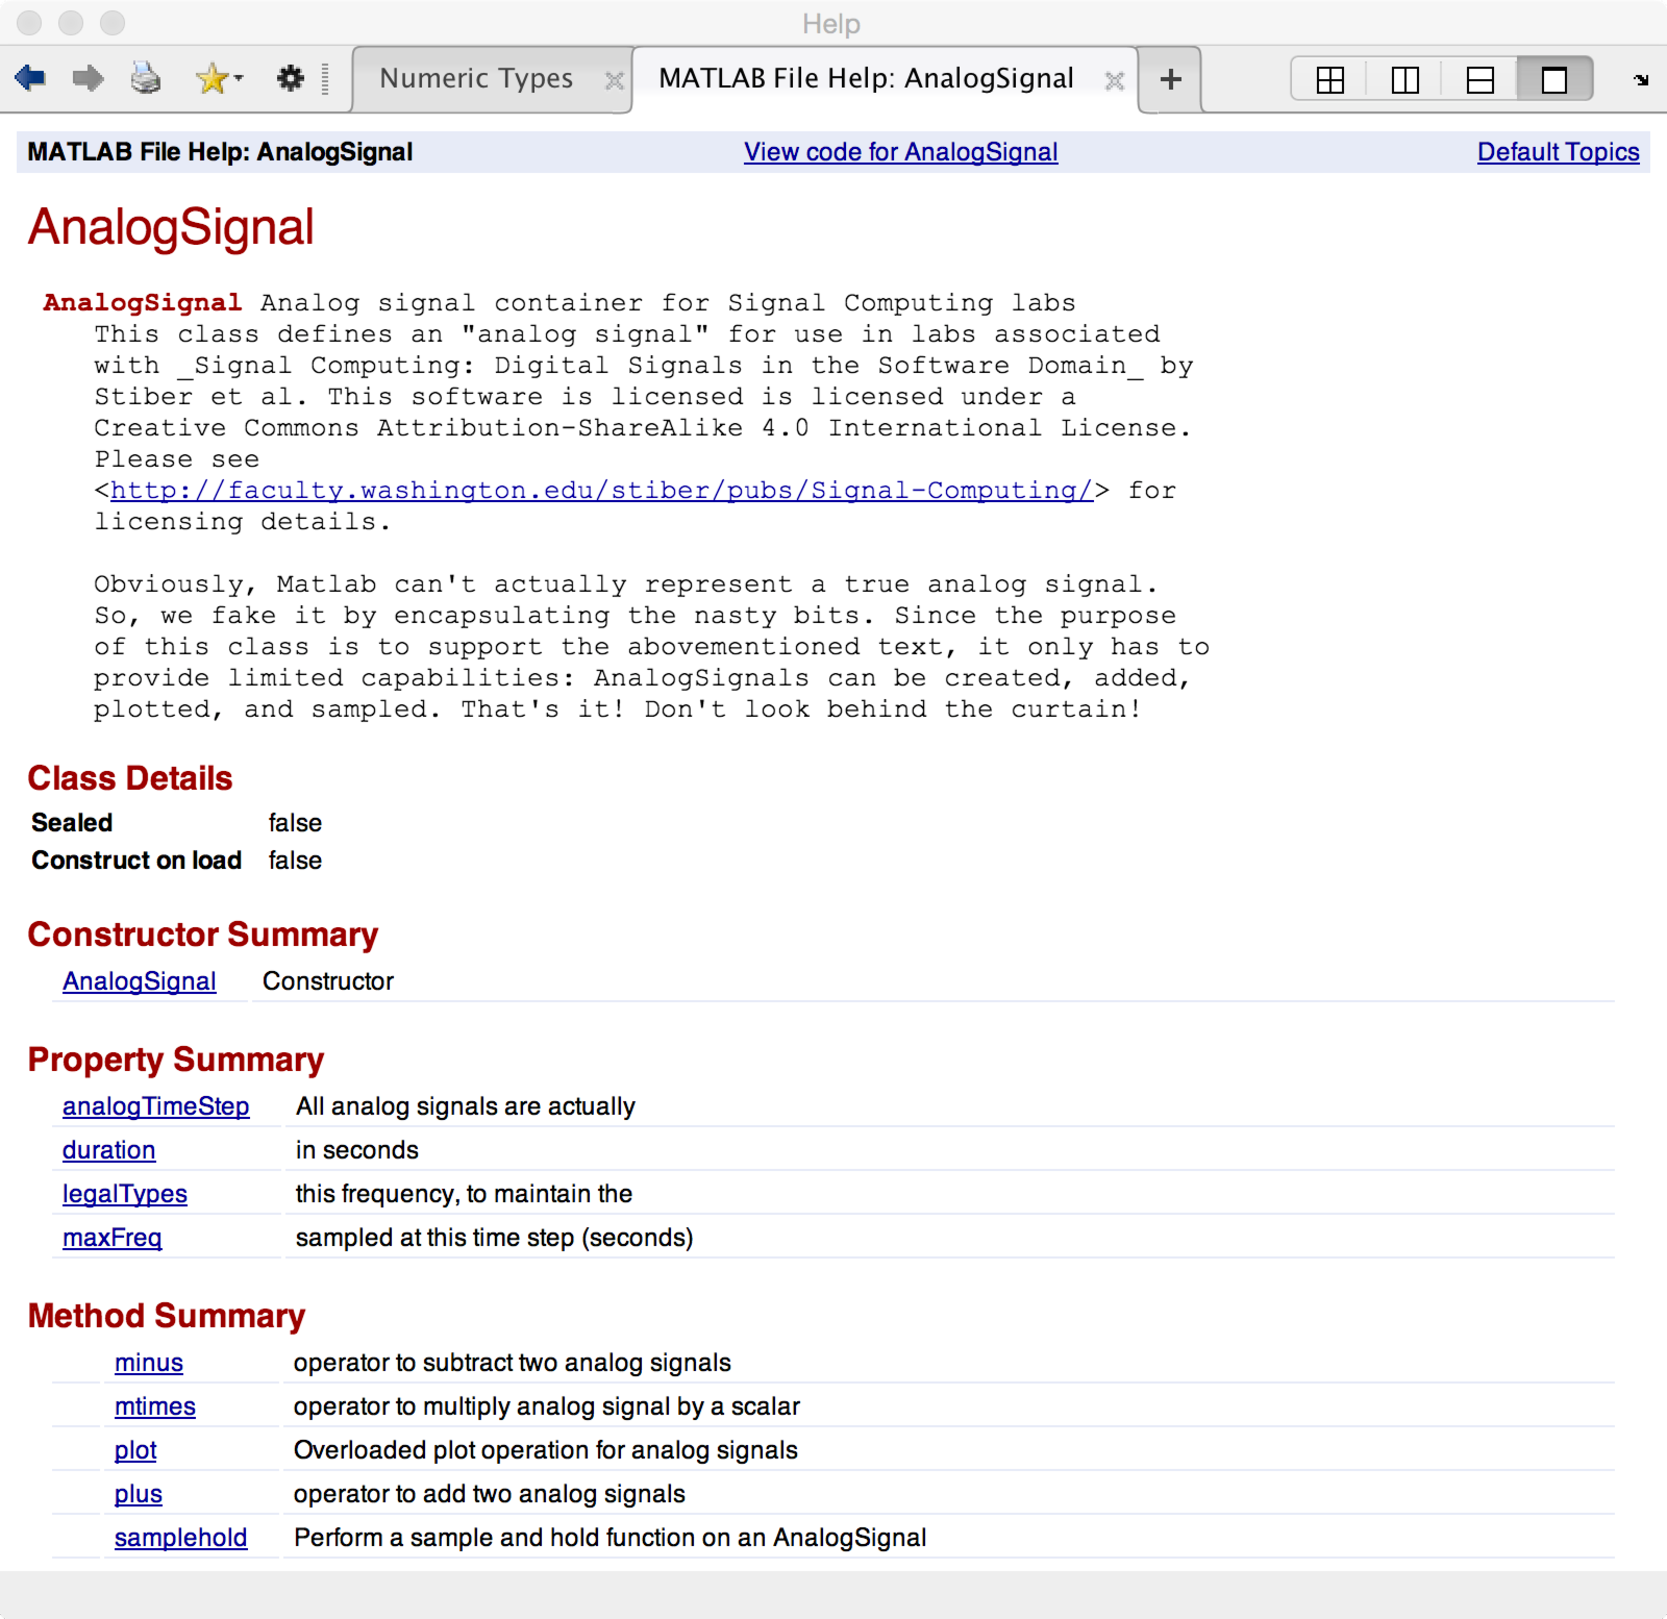
\includegraphics[width=0.75\textwidth]{lab1/AnalogSignal-help}
\end{center}
\caption{Example help screen for the \texttt{AnalogSignal}
  class. This example may be out-of-date; use the Matlab
  \texttt{doc AnalogSignal} command to get current
  documentation.\label{fg:analogsignal-help}}
\end{figure}

Information hiding is used in our implementation of analog signals. We
make use of the object-oriented programming aspects of Matlab to
create an \texttt{AnalogSignal} class. If you look up the
documentation for \texttt{AnalogSignal} (using
\verb|doc AnalogSignal|), you'll see something like
figure~\ref{fg:analogsignal-help}. The key operations on these analog
signals are:
\begin{itemize}
\item Creating an analog signal (ex: \texttt{a =
    AnalogSignal('sawtooth', 2.0, 1.0, 10.0)}).
\item Scaling an analog signal (ex: \texttt{b = a * 5})
\item Adding two analog signals (ex: \texttt{c = a + b})
\item Subtracting two analog signals (ex: \texttt{d = c - a})
\item Plotting an analog signal (ex: \texttt{plot(d)})
\item Sampling an analog signal (ex: \texttt{x = d.samplehold(0.1)})
\end{itemize}

You will get a lot more experience working with analog signals shortly
in this class, so for the time being just play with this a bit.


%&LaTeX

% Sections of this are duplicated from the DSP First labs 1a and
% 1b. Those sections MUST be rewritten before this can be released
% externally.


\section{Complex Exponentials in J-DSP}

% TODO: redo this beginning section to introduce the idea of a time
% series in JDSP relate the rotating phasors addition to moving back
% and forth along the real axis.  Scrap the MATLAB introductions in
% favor of introducing how to look at phasors in JDSP intuitively and
% that the complex plane is just a succinct way of looking at sine
% waves.

In this lab you will be investigating how complex exponentials relate
to sine and cosine waves. Once completed you should have a feel for
how the complex plane can be used to represent \textit{real,
  oscillating functions} (like sines and cosines). Moreover, you
should have an appreciation for why it is easier to mathematically
manipulate and analyze oscillating functions using complex
arithmetic. We will be using J-DSP exclusively to illustrate key
concepts of how complex numbers can represent frequency.

\subsection{Complex Vectors and Exponentials in J-DSP}
\label{sc:jdsp-sines}
In this section you will use J-DSP to generate vectors and phasors in the complex plane. Specifically, you will relate changes in the complex plane to changes in the time domain.

% Complex Vector in J-DSP
\begin{figure}[t]
  \begin{center}
    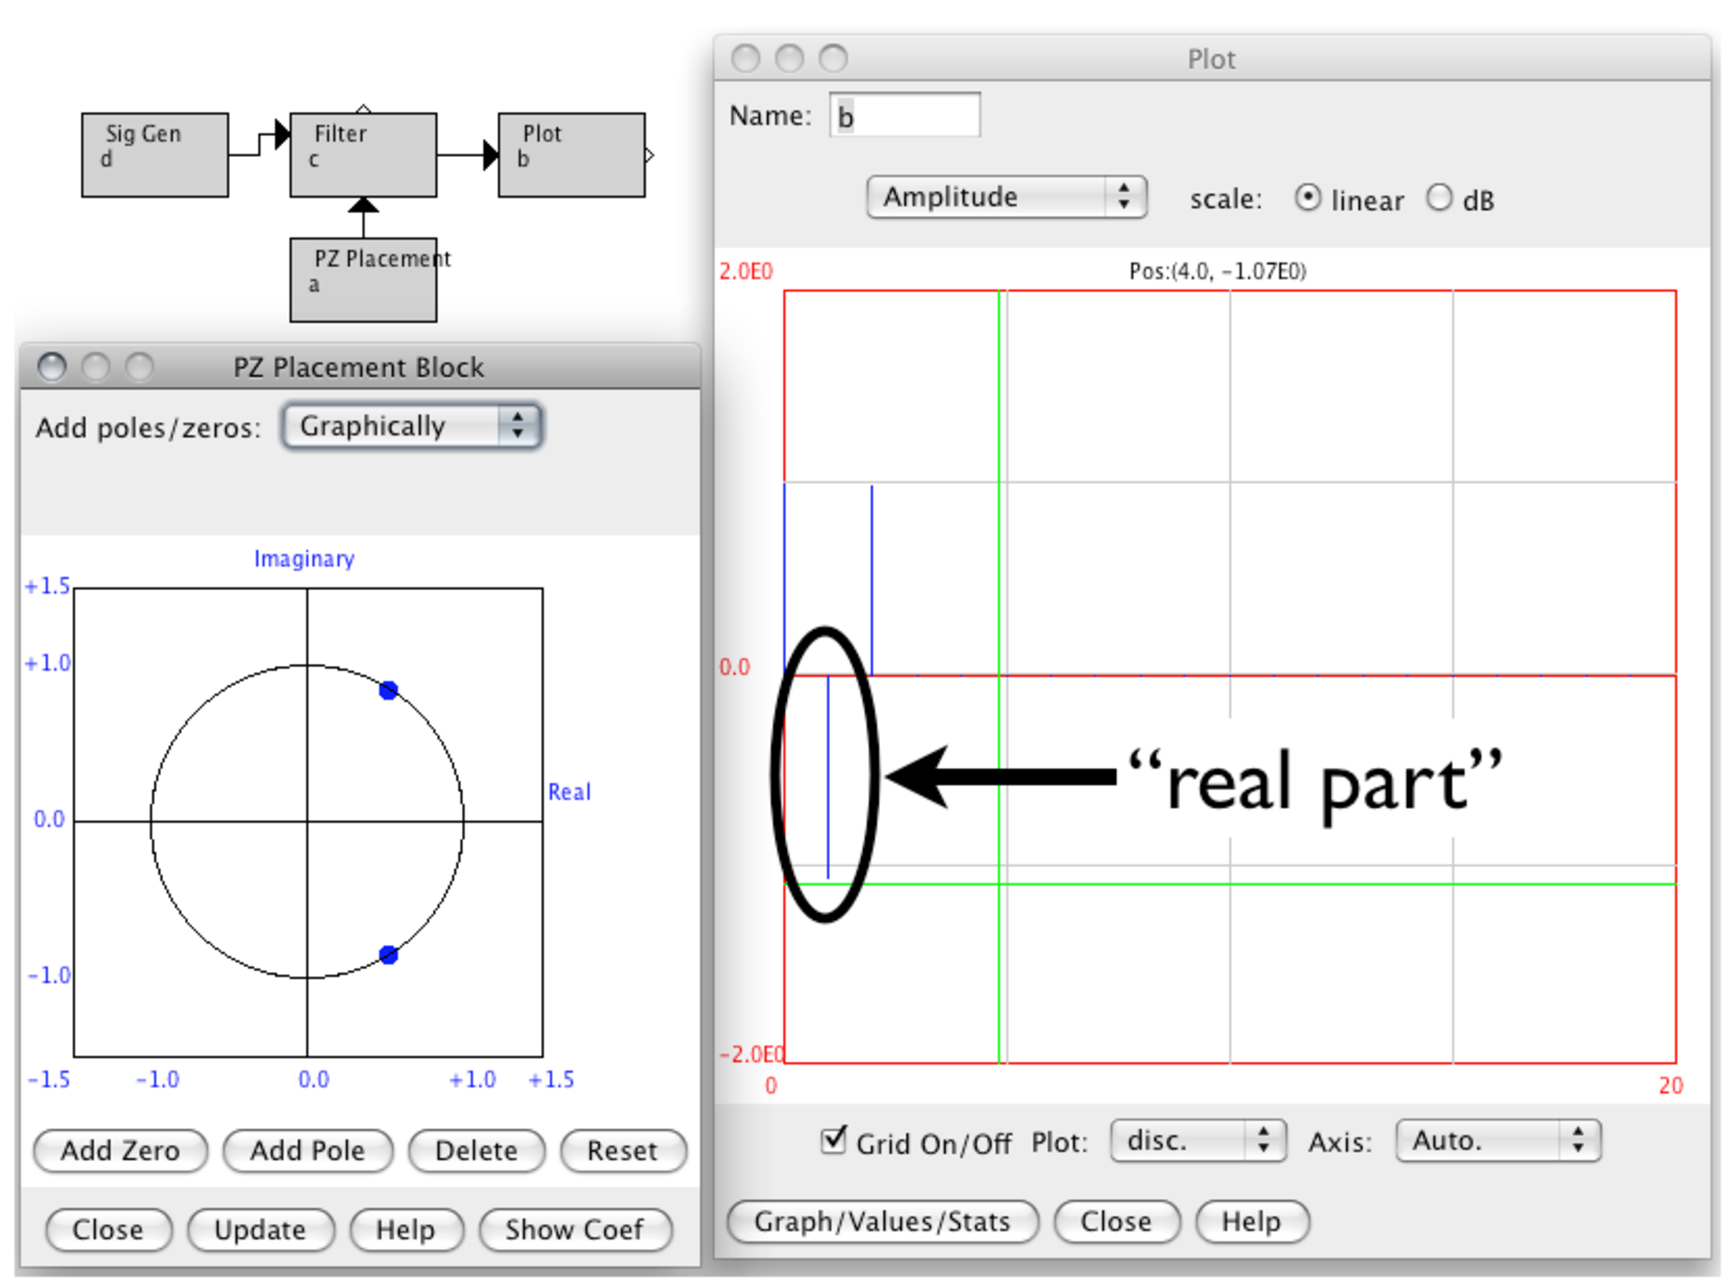
\includegraphics[height=3in]{lab2/PoleZeroAsComplexVector}
  \end{center}
\caption{J-DSP setup for simulating a two vectors that add to be a real output, represented as sample 2 in the plot.\label{fg:PoleZeroAsComplexVec}}
\end{figure}

% idea of the vectors in the complex plane
\paragraph{Step 1.1} 
WARNING: The next step will overwrite any work not saved in J-DSP. Use the given script to generate the diagram in Figure \ref{fg:PoleZeroAsComplexVec}. Download: \url{http://faculty.washington.edu/stiber/pubs/Signal-Computing/jdsp-scripts/polezero_as_vector.txt}.

Use the \menu{File} $\rightarrow$\menu{Import from Script...} command in the J-DSP window and copy the text  over. You should see a block diagram similar to that in Figure \ref{fg:PoleZeroAsComplexVec}. If you do not, there was a failure loading the script, exit out of J-DSP, and try again. 
This script provides an interactive way to \textit{view vectors} in the complex plane and what they look like in the time domain. We are not yet ready to talk about every block in the J-DSP diagram. However, two blocks are of interest to us now. We will interact with \block{PZ-Placement} (block a) and \block{Plot} (block b). Open the dialog for the \block{Plot} block in the diagram if it is not already active. You should see three discrete points in the output plot (Figure \ref{fg:PoleZeroAsComplexVec}). 

Now open the dialog for \block{PZ-Placement} if it is not already active. You should see a plot of the complex plane with two $\circ$ marks on it and a large black circle that represents the unit circle. This \block{PZ-Placement} block is normally used for filter design, but we will be using it to represent a vector in the complex plane, $Re^{j\phi}$. If you drag the $\circ$ marks in \block{PZ-Placement}, you can change the amplitude and phase of the vector and view the ``real part'' of the output in the time domain plot. When you do this, you will also see the three points in the output plot change in magnitude. We will be interested in what happens to the middle value in the plot (marked ``real part'' in Figure \ref{fg:PoleZeroAsComplexVec}). You can (1) click and drag or (2) you can enter the real and complex values manually using the \button{Graphically} and \button{Manually} selections from the pop-up menu. 
Note that the \block{PZ-placement} block is doing more than just helping to plot the ``real part'' of the complex vector. For now, just know that the second point plotted in the \block{Plot} dialog corresponds to the ``real part''  of the complex vector. It is directly affected by the magnitude and phase of the vector. For the following questions, recall that a phasor is just a spinning vector in the complex plane.  

\begin{enumerate}
\item If you repeatedly drag the $\circ$ marks in a circular motion along the black circle in \block{PZ-placement}, what happens to the ``real part'' in the plot dialog? If you were to keep the vector magnitude constant and graph the ``real part'' of the plot over time as it moves around the complex plane, would you expect to see a sinusoidal wave? How would the amplitude and phase of the sinusoidal wave be affected by the complex vector?

\end{enumerate}


% Complex Phasor in J-DSP
\begin{figure}[t]
  \begin{center}
    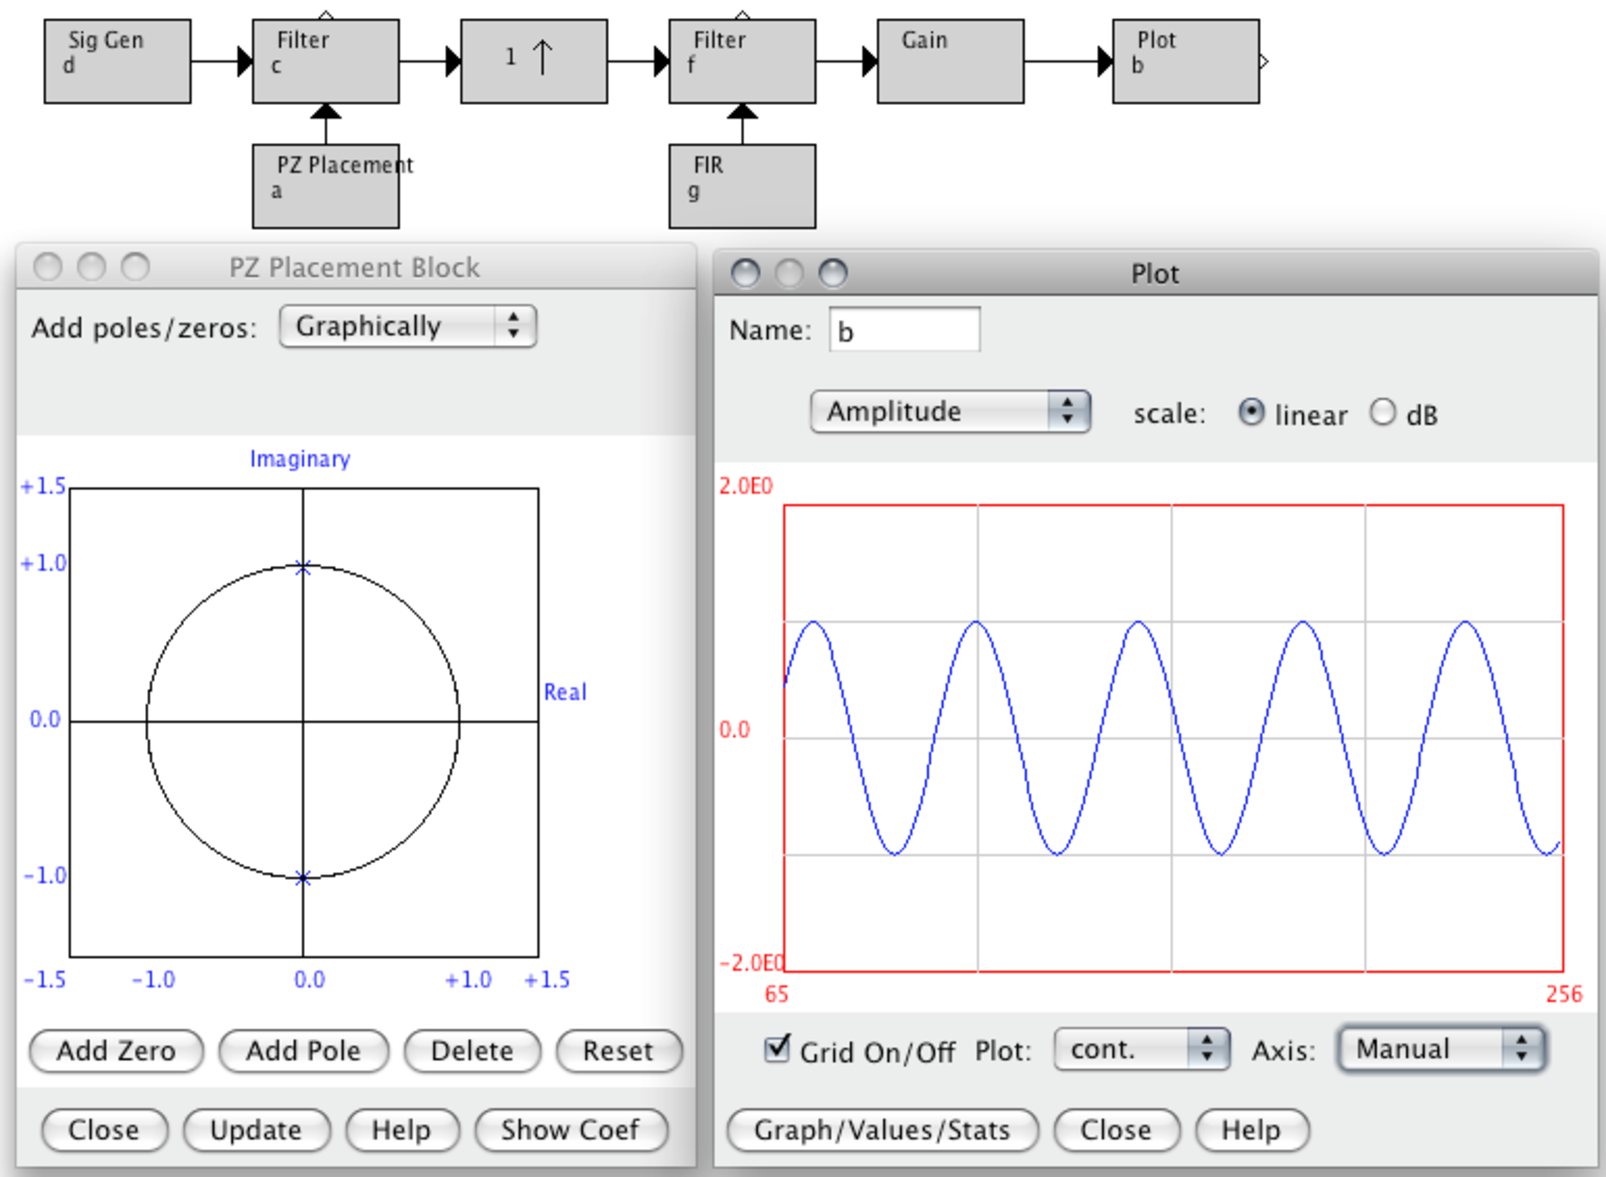
\includegraphics[height=3in]{lab2/PoleZeroAsComplexExp}
  \end{center}
\caption{J-DSP setup for simulating two phasors that add to be a real sinusoid.\label{fg:PoleZeroAsComplexExp}}
\end{figure}

% introduce the pole zero placement as means of visualizing the phasor (only a weak analogy, it would be great to have a built-in J-DSP phasor animation function)
\paragraph{Step 1.2} 
WARNING: The next step will overwrite any work not saved in J-DSP. Use the given script to generate the diagram in Figure \ref{fg:PoleZeroAsComplexExp}. Download: \url{http://faculty.washington.edu/stiber/pubs/Signal-Computing/jdsp-scripts/polezero_as_phasor.txt}. 

Use the \menu{File} $\rightarrow$\menu{Import from Script...} command in the J-DSP window and copy the text  over. You should see a block diagram similar to that in Figure \ref{fg:PoleZeroAsComplexExp}. If you do not, there was a failure loading the script, exit out of J-DSP, and try again. 

This script provides an interactive way to manipulate the \textit{frequency} of phasors in the complex plane and view the sinusoidal output. We are not yet ready to talk about every block in the J-DSP diagram. Like before, two blocks are of interest to us now. We will interact with \block{PZ-Placement} (block a) and \block{Plot} (block b). Open the dialog for the \block{Plot} block in the diagram if it is not already active. You should see a cosine wave. (Note that, in the plot in the figure, the limits of the $X$-axis have been changed manually to have a lower limit of 65, rather than zero. Unfortunately, the axis limits don't get restored when a script is imported, so you will see the auto axis limits, rather than the ones set as in the figure. You can set the limits in the plot to match the figure yourself.)

Now open the dialog for \block{PZ-Placement} if it is not already active. This block is normally used for filter design, but we will be using it to simulate a phasor in the complex plane. Recall that a phasor can be represented in polar form as $Re^{j\omega t}$ where $\omega $ represents the frequency at which the phasor rotates and $R$ represents the magnitude. Dragging the \texttt{x} marks in \block{PZ-Placement} lets you change the $\omega $ of the resulting phasor and view the sinusoid in real time. Note that you can also change the magnitude of the complex phasors in the dialog, but this is not the same as changing the amplitude of a complex phasor. There are other things going on in this block that we are not ready to talk about - we are actually treating something called a ``pole'' as a rotating phasor, which is not quite right. For now, try to keep the magnitude of the phasor as close to ``one'' as possible (i.e., try to keep the \texttt{x} on the black line representing the unit circle). 

\begin{enumerate}
\item Drag the phasors along the unit circle towards the (1,0) point (where the unit circle meets the real axis in the right half plane). What happens? What happens when you move away from the the (1,0) point along the unit circle? Include a screenshot of the \block{Plot} and \block{PZ-placement} dialogs in your lab report.


\item Notice that you cannot move only one of the phasors. You must move both at the same time. Does it make sense that you must move both symmetrically? Why or why not? \textit{Hint:} think about the output as being the rotating phasors $e^{j\omega_1 t}+e^{j\omega_2 t}$, where $\omega_1$ and $\omega_2 $ are proportional to the angles of the ``poles.''

\end{enumerate}


\subsection{Complex Exponentials}

\paragraph{Step 2.1} Compute the following complex arithmetic by hand:
\begin{enumerate}\renewcommand{\theenumi}{\alph{enumi}}
\item What is the complex conjugate of $z_1 = -1 + j 0.3$?

\item Let $z_2 = 1 + j 0.6$ What is $z_1 + z_2$?

\item What is $z_1 - z_2$?

\item What is $z_1 z_2$?

\item What is $z_2/z_1$?

\end{enumerate}

\paragraph{Step 2.2} Compute or prove the following using complex arithmetic and Euler's Formula by hand. Recall that Euler's Formula is given by: $e^{\pm j\omega t}=\cos(\omega t) \pm j \sin(\omega t)$.

\begin{enumerate}
\item A complex number can be written in rectangular coordinates as $z
  = x + j y$. Write the relations to calculate the polar form, $z=(r,
  \theta)$ or $z = r e^{j\theta}$.

\item Using Euler's formula, express $\cos x$ and $\sin x$ as a
  combination of complex exponentials.
  
\item Convert $\cos(\omega t+\phi)$ into the sum of complex exponentials.  

\item Find expressions for 1, $j$, $1 + j$, $(1 + j\sqrt{3})/2$ as
  complex exponentials.

\item Compute $[(1+j\sqrt{3})/2]^2$ and $(1+j)^4$ directly (using the
  rectangular representations).
  
\item Compute $[(1+j\sqrt{3})/2]^2$ and $(1+j)^4$ using complex
  exponentials.
  
\end{enumerate}


\paragraph{Step 2.3} Prove the following regarding complex conjugates:

\begin{enumerate}
\item Show that $(z_xz_y)^* = z_x^* z_y^*$.

\item Express $|z|^2$ as a function of $z$ and $z^*$.

\end{enumerate}




\subsection{Complex Exponentials in J-DSP}

\paragraph{Step 3.1} In this step, you are asked to use JDSP
to create a block diagram capable of synthesize a waveform of the form:
$\cos(2\pi (200) t+\phi_1) + \cos(2\pi (200) t +\phi_1) +\cos(2\pi (200) t+\phi_1) +\cos(2\pi (200) t+\phi_1) $
And plot the output of each cosine wave and their sum. Use the \block{Cont. Signal} and \block{Analog Adder} blocks in the ``Analog Blocks'' function set. Include a screenshot of the block diagram in your writeup. Use this diagram to complete Step 3.2.


\paragraph{Step 3.2} Generate four sinusoids with the following
amplitudes and phases (remember to convert from rad/s to Hz and from radians to degrees):
\begin{align}
x_1(t) &= 5 \sin(2\pi(200)t +0.5\pi) \\
x_2(t) &= 5 \sin(2\pi(200)t - 0.25\pi) \\
x_3(t) &= 5 \sin(2\pi(200)t +0.4\pi) \\
x_4(t) &= 5 \sin(2\pi(200)t - 0.9\pi) 
\end{align}

\begin{enumerate}\renewcommand{\theenumi}{\alph{enumi}}
\item Make a plots of all four signals in J-DSP. 

\item Verify that the phase of all four signals is correct at $t = 0$,
  and also verify that each one has the correct maximum amplitude. Use
  the \block{Analog Plot} blocks.

\item Create the sum sinusoid,
  $x_5(t)=x_1(t)+x_2(t)+x_3(t)+x_4(t)$. Make a plot of $x_5(t)$ over
  the same range of time as used in the last plot. Include your plot in your writeup 
  
\item Using pencil and paper: Express   $x_1(t)$ through $x_4(t)$ as complex exponentials. 
  
	
\item Using pencil and paper: Express   $x_5(t)$ as a sum of complex exponentials. 	


\item Using complex exponentials, express the amplitude and phase of $x_5(t)$ (use pencil and paper with the aide of a graphing calculator, spreadsheet, or MATLAB).


\end{enumerate}



% LocalWords:  MATLAB DSP

%&LaTeX

\section{Signals in the Computer}

In this lab, you will use JDSP to explore how a physical signal can
be considered to be composed of a sum of sinusoids --- its
\emph{Fourier series}. You will then investigate how capturing this
signal for computer use --- sampling and quantization --- modifies the
signal. Finally, you will see how the choices you make in the
parameters for sampling and quantization affect the quality of the
digitized, computer signal. 



\subsection{Fourier series representation of a physical signal}
	In this section, you will use the  \block{Cont Sig} block in J-DSP to simulate a analog signal 
	generator. The \block{Cont 
	Sig} block is capable of simulating analog signals of varying frequency content. 
	
	% Block diagram, step 1
	\begin{figure}[b]
	  \begin{center}
	    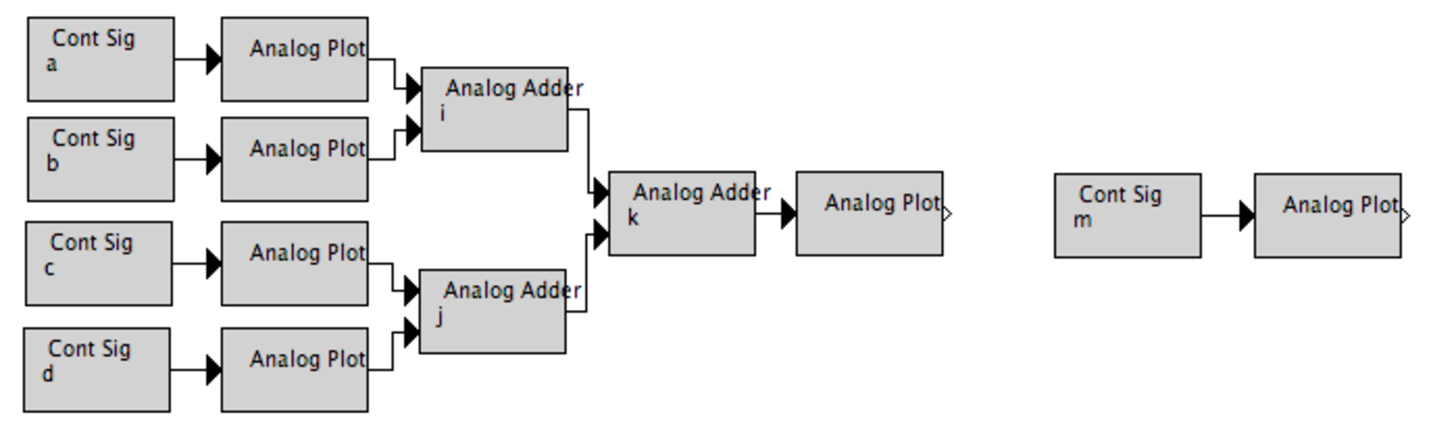
\includegraphics[height=1.5in]{lab3/block_diagram_step1}
	  \end{center}
	\caption{ A J-DSP diagram for summing and plotting analog sine waves (left) and a single 
	triangle wave (right). 
	\label{fg:step1}}
	\end{figure}

\paragraph{Step 1.1} Create a J-DSP diagram that sums together four continuous time sinusoids 
	and plots their sum. Use the ``Analog Blocks'' function set and the \block{Adder} block only (See 
	Figure \ref{fg:step1}). Also create a separate set of blocks that plots a continuous time triangle 
	wave at a \option{frequency} of 200 Hz and \option{amplitude} of 1. In the next section you will 
	simulate this triangle wave using the sum of sinusoids.

\paragraph{Step 1.2} Recall that any periodic signal can be represented as a sum of harmonic 
	sinusoids. The amplitude of each harmonic is known as the Fourier Series. It may at first seem
	like sums of sinusoids would be poor approximations of real periodic signals, but this is not 
	the case. We
 	can illustrate this using a triangle wave. The formula for synthesis of a triangle wave with 
	frequency $\omega_0$ is a sum of harmonically related sine waves (its Fourier series):
	\[
	x(t) = \sum_{k=0}^{\infty}
	\left( 
	\underbrace{ \frac{8}{\pi^2} \frac{(-1)^k}{(2k+ 1)^2} }_{ \text{amplitude} } 
	\underbrace{ \sin((2k+1)\omega_0 t) }_{ (2k+1)^{th}\text{ harmonic} } 
	\right)
	\]
	In this case, in the analog domain, we are dealing with frequencies in
	Hz, and so $\omega_0 = 2\pi f_0$. Notice that the Fourier Series of the triangle wave only uses 
	odd harmonics (i.e., the only non-zero frequencies are $(2k+1)\omega_0=\omega_0, 3\omega_0, 
	5\omega_0 \cdots$). Also notice that resulting wave will be zero mean because there is no ``DC'' 
	term (i.e., $2k+1 \neq 0$ for any integer k). 
	Use your diagram from Step 1.1 to generate and sum the
	first 7 harmonics of the Fourier Series of a triangle wave and plot the resultant signal (i.e., use 
	$f_0$, $2f_0$, $3f_0$, $\cdots 7f_0$, where $f_0=$200 Hz). How does this signal compare to 
	the triangle wave computed directly in \block{Cont. Sig}?
	

\paragraph{Step 1.3} Another way to view a signal is in the \emph{frequency domain}. For a 
	signal expressed in terms of its Fourier Series, the \emph{frequency domain} representation
	is merely the coefficients of the harmonics. Use your favorite spreadsheet or plotting tool to 
	compute and plot 
	the spectrum of a triangle wave.  Note that you are \emph{not} being asked to plot the triangle 
	wave as a function of time; you should plot the amplitudes of the Fourier Series as a 
	function of the harmonics' frequencies (like the vertical lines in textbook figure~1.12).  
	


\subsection{Sampling}

The first step in digitization is \emph{sample and hold}, in which the
continuous analog signal is converted to a \textit{discrete-time}
analog signal (an analog signal that only changes its value at
particular points in time). You will use the \block{Sample-Hold} block
in J-DSP to simulate this.

% Block diagram, step 2
\begin{figure}[h]
  \begin{center}
    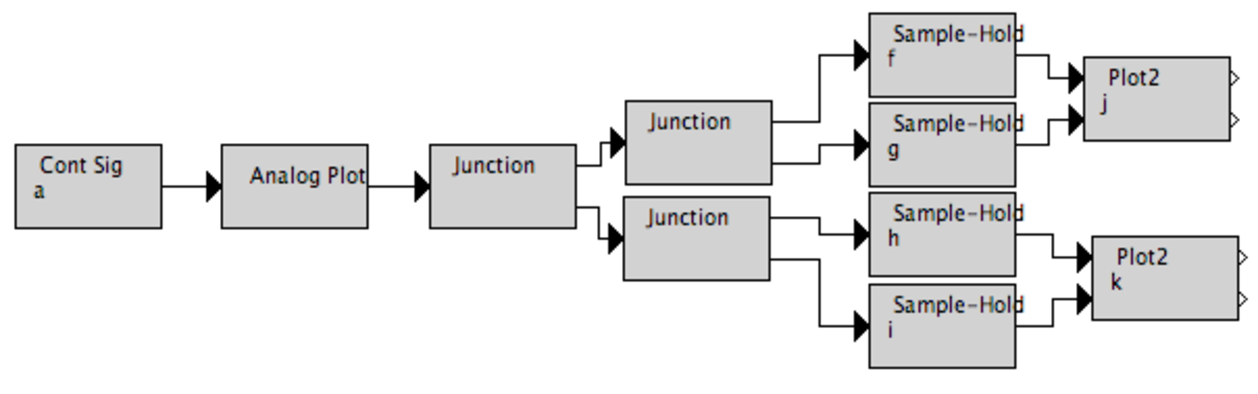
\includegraphics[height=1.5in]{lab3/block_diagram_step2}
  \end{center}
  \caption{ A J-DSP diagram for investigating sampling rate. \label{fg:step2}}
\end{figure}

\paragraph{Step 2.1} Create an \block{Cont Sig} sine waveform ranging
from -5 to 5V with a frequency of 200Hz (Figure \ref{fg:step2},
leftmost block).

\paragraph{Step 2.2} Use four \block{Sample-Hold} blocks to sample
this signal at 300Hz, 500Hz, 1000Hz and 2000Hz. Plot the original and
all four sampled signals separately (Figure \ref{fg:step2}). Clearly,
the results are not the same, and none look identical to the original
sine wave. What are the two essential pieces of information about a
sine wave that need to be preserved when sampling it?  Does it appear
that all sampled versions are equally useful in achieving this? Why or
why not (in other words, your answer to this question should not be
just ``yes'' or ``no'')?


\subsection{Analog to Digital Conversion}

	The last step of digitization is called ``analog to digital conversion,'' or \emph{quantization}. In 
	this step, the sampled analog signal is converted to a discrete signal, with values represented 
	by $b$ bit integers. We will use the \block{Quantizer} block under the ``Statistical DSP'' function 
	set to perform this conversion.
	
	% Block diagram, step 3
	\begin{figure}[h]
	  \begin{center}
	    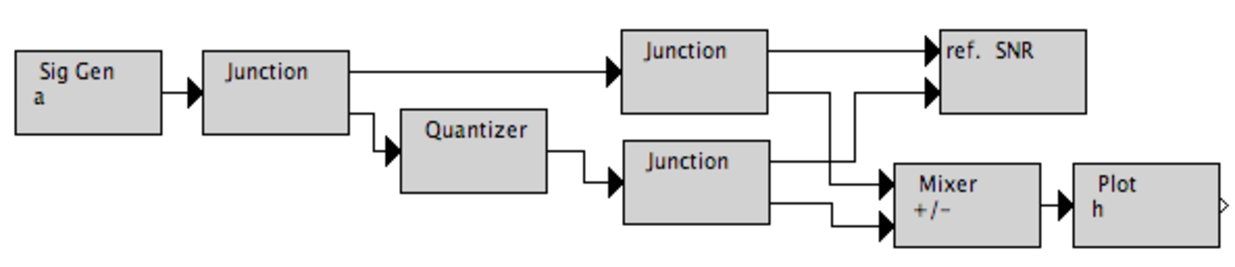
\includegraphics[width=5.0in]{lab3/block_diagram_step3}
	  \end{center}
	\caption{ A J-DSP diagram for investigating quantization error and calculating SNR. 
	\label{fg:step3}}
	\end{figure}

\paragraph{Step 3.1} Next we will be using the \block{SNR} block under the ``Basic Blocks'' 
	function set to compute signal-to-noise ratio (SNR) as a result of quantization. Place the 
	\block{SNR} block and open the dialog associated with it. You will see the equations used to 
	calculate the numerator and denominator. In your own words, what quantity is calculated in the 
	numerator and what quantity is calculated in the denominator of this ratio (Hint: can you 
	describe the values in terms of \emph{root mean square} (RMS) values)? Note that this SNR is 
	different than what we did in the textbook, because we are now doing the computation for a 
	\textit{specific} signal, not just figuring SNR for a possible \textit{range} of signal values.
	

\paragraph{Step 3.2} Use the J-DSP diagram in Figure \ref{fg:step3} to compute the SNR for a 
	quantized sinusoid. Use the \block{SigGen} block with a ``amplitude'' of 5, ``frequency'' of 0.05$
	\pi$, and ``Pulsewidth'' of 256. Use 2, 4, 8, 12, and 16 bits quantization. Use your favorite 
	spreadsheet or plotting software to plot SNR versus number of quantization bits (i.e., a scatter 
	plot). Use the output of \block{SigGen} as reference for the \block{SNR} block. 

\paragraph{Step 3.3} Plot the quantization error by using the \block{Adder} block (bottom right 
	blocks of Figure \ref{fg:step3}). Set the \block{Adder} block to ``subtract'' by opening the dialog 
	and switching the ``$+$'' sign to ``$-$.'' You only need to include the quantization error plot for 
	``4 bits'' in your report (but be sure to view the error plots for all quantization levels).

\paragraph{Step 3.4} Repeat Step 3.2 using a triangle waveform with ``Gain'' of 5 and 
	``Pulsewidth'' of 256. 

\paragraph{Step 3.5} As you double the number of bits used in quantization, how does the SNR 
	change? Refer to specific features of your plots from Steps~3.2--3.4 to justify your answer. 
	

% LocalWords:  WebQ MATLAB

%&LaTeX

\section{Feed It Forward}

This lab covers the basic concepts of filtering and feedforward filters. 
You may have also heard of feedforward filters referred to as 
finite impulse response (FIR) filters. In this lab, we will cover the basic idea
of a filter, its mathematical representation (such as the defining equation,
frequency response, and transfer function), the relationship among
filter coefficients, zero placement, and filter type (low pass, high
pass, band reject), and some basic properties of filters.


\subsection{Overview of Filtering and Matlab}

A \emph{digital filter} is a signal processing operation that can be
  described equivalently by its \emph{defining
  equation}, \emph{transfer function}, or \emph{frequency response}. 
  Each representation completely defines the filter. It is advantageous 
  to use each of the different representations depending on whether you are
  \emph{implementing}, \emph{analyzing}, or \emph{designing} an FIR filter:
\begin{eqnarray*}
  y[n] &=& \underbrace{\sum_{k=0}^M b_k x[n-k]}_{\text{defining equation}} \\ 
  \hline \\
  Y &=& H(z) X\\
  H(z) &=& \underbrace{\sum_{k=0}^M b_k z^{-k}}_{ \text{transfer function} } \\
  \hline \\
  Y &=&  \mathcal{H}({\hat{\omega}}) X \\
  H(e^{j\hat{\omega}})  = \mathcal{H}({\hat{\omega}}) 
  &=& \underbrace{\sum_{k=0}^M b_k e^{-j \hat{\omega}k}}_{\text{frequency response}} 
\end{eqnarray*}

In these equations, $x[n]$ and $y[n]$ are the $n^\mathrm{th}$ samples
from the input and output, respectively, while $X$ and $Y$ represent
the entire input and output signal (all of the samples in the
signal). A $k$-sample time delay of a signal is produced by
multiplication by the delay operator, $z^{-1} = e^{-j
  \hat{\omega}k}$. In all three cases (but most simply for the
transfer function), we can obtain insight into the filter's operation
from the \emph{coefficients}, $b_k$. We can do this by factoring the
transfer function polynomial: its roots are the \emph{zeros} of the
filter and they can be real or complex.  The placement of the zeros in
the complex plane (most usefully expressed in polar coordinates) will
tell us which frequencies are suppressed and to what extent those
frequencies are suppressed (we can calculate each using the angle and
magnitude of the zero, respectively).

Matlab has a modest set of functions related to filtering (a much more
substantial set of tools comes along with the Matlab Signal Processing
Toolbox, but we will confine ourselves here to using core Matlab). The
\verb|filter| function applies a general digital filter to a
signal. For this lab, we will stick using this filter as follows:
\begin{lstlisting}[style=Matlab-editor,basicstyle=\mlttfamily\small]
a = [1];              % This will be relevant later for feedback filters
b = [b0 b1 b2];       % Coefficients (remember, Matlab indices start at 1)
y = filter(b, a, x);  % x is input signal; y is output
\end{lstlisting}
This allows us to define the $b_k$ coefficients for a filter and provide
them to the filter function as a vector so that it can filter the
input signal.

We'd also like to specify a feedforward filter by indicating its zero
locations, which we can do by using the \verb|poly| function to
compute the coefficients from a set of roots. So, for example, if we
want a feedforward filter with zeros at $0.9 + 0j$ and $0.75e^{\pm j
\pi/4}$, we can compute the $b_k$ values as:
\begin{lstlisting}[style=Matlab-editor,basicstyle=\mlttfamily\small]
r = [ (0.9 + 0.0*j) (0.75*exp(j*pi/4)) (0.75*exp(-j*pi/4))];
b = poly(r);
a = [1];
y = filter(b, a, x);
\end{lstlisting}
(Where the definition of \verb|r| is written a bit more verbosely than
it has to be.) Note that, from the documentation for \verb|poly|, the
vector of coefficients it produces are ordered from highest to lowest
powers; this corresponds to the same order as the coefficients in the
\verb|b| vector, after dividing by $z^{-M}$, the highest delay
term.

You can visualize the zero locations with the following code:
\begin{lstlisting}[style=Matlab-editor,basicstyle=\mlttfamily\small]
plot(r, 'o')
rectangle('Position', [-1 -1 2 2], 'Curvature', [1 1])
line([-1 1], [0 0], 'Color', [0 0 0])
line([0 0], [-1 1], 'Color', [0 0 0])
axis equal
\end{lstlisting}
Here, we use the unfortunately named \verb|rectangle| function
to draw the unit circle and the \verb|line| function to draw the real
and imaginary axes.

Finally, you can compute and plot the magnitude of the filter's
frequency response pretty directly in Matlab:
\begin{lstlisting}[style=Matlab-editor,basicstyle=\mlttfamily\small]
omegahat = [0: 0.01: pi];   % define the frequency axis
z = exp(j*omegahat);        % define the complex frequency axis
H = polyval(b, z);          % evaluate the transfer function polynomial
plot(omegahat, 20*log10(abs(H)/max(abs(H))));
xlabel('$\hat{\omega}$, radians','Interpreter', 'latex');
ylabel('$|\mathcal{H}(\hat{\omega})|$, dB','Interpreter', 'latex')
\end{lstlisting}
You'll note that the code above plots the ratio of the magnitude of
the frequency response to the maximum value of that magnitude. This is
done because it is convention to ignore whether a filter amplifies a
signal overall; what we are concerned with are the relative amounts
that different frequencies are passed or blocked.


Remember, we can define a specific filter using either of the methods
above. Sometimes it is easier to understand the filter using zeros and
sometimes it is easier to use the coefficients directly.  Either
method can be used to represent the same filter, and we can go back
and forth with the \verb|poly| and \verb|roots| functions (and back
and forth between polar and rectangular representations of complex
numbers with the \verb|abs|, \verb|angle|, and \verb|exp| functions).


\subsubsection{From Filter Coefficients to Transfer Function and Frequency Response}

Given the coefficients of an FIR filter we can solve for the zero
locations and the frequency response.  For example the two-point
averaging system is given by:
\begin{equation}
y[n] = \frac{1}{2}x[n] + \frac{1}{2}x[n-1]
\label{eq:two-point-filter}
\end{equation}
we can find the transfer function by rewriting the filter using the
delay operator, $z$:
\begin{eqnarray}
  Y    & = & \frac{1}{2} X + \frac{1}{2} z^{-1} X \\
  H(z) & = & \frac{Y}{X} = \frac{1}{2} (1 +  z^{-1})
\end{eqnarray}
If we're interested in the \emph{zero location} we can then multiply
$H(z)$ by $z/z$ to obtain:
\begin{equation}
  H(z) = \frac{\frac{1}{2} (z + 1)}{z}
\end{equation}
The root of the numerator, $z=-1$ is the location of the only zero
(the root(s) of the denominator for an FIR filter are always at $z=0$,
and do not affect the frequency response). We can also derive the
frequency response from this by remembering that $H(e^{j\hat{\omega}})
= \mathcal{H}({\hat{\omega}})$ or that $z=e^{j\hat{\omega}}$. From the
zero location, $z=-1$, we can immediately tell that the frequency
response is zero at $e^{j\hat{\omega}}=-1$ or $\hat{\omega}=\pi$. With
a zero at an angle of $\hat{\omega}=\pi$, this is a low-pass
filter. As a warm-up, use Matlab and the coefficients of
equation~\ref{eq:two-point-filter} to verify the expected zero
placement and frequency response.

\subsubsection{From Zero Placement to Filter Coefficients}

When we are given the zero placement, we can very easily determine the
filter coefficients because those zeros are the roots of a factored
polynomial. For example, given two complex conjugate zeros, $z_1$ and
$z_2$ (i.e., the real parts are equal, $\Real[z_{1}] = \Real[z_{2}] =
\Real[z_{1,2}] $, and the imaginary parts are negatives of one another
$ \Imag[z_{1}] = -\Imag[z_{2}] $ or, equivalently in polar
coordinates, $z_{1} = r e^{j\hat{\omega_0}}$ and $z_{2} = r
e^{-j\hat{\omega_0}}$), the transfer function is:
\begin{eqnarray}
  H(z) & = & (z - z_1)(z - z_2)/z^2 \\
  & = & (z^2 - (z_1 + z_2) z + z_1 z_2)/z^2 \\
  & = & 1 - 2 \Real[{z_{1,2}}] z^{-1} + r^2 z^{-2} \\
  & = & 1 - 2 \Real[r(\cos(\omega_0) \pm j\sin(\omega_0))] z^{-1} + r^2 z^{-2} \\
  & = & \underbrace{1}_{b_0} -\underbrace{2 r\cos(\omega_0)}_{b_1} z^{-1} + \underbrace{r^2}_{b_2} z^{-2}
\end{eqnarray}
At this point, we can rewrite the transfer function as the filter's
generating equation, using the delay operator $z^{-k}$, $y[n] = x[n] -
2 r\cos(\omega_0)x[n-1] + r^2 x[n-2]$. This allows us to read off the
filter coefficients: $b_0 = 1$, $b_1 = -2 r\cos(\omega_0)$, and $b_2 =
r^2$.

\subsection{Frequency Response and Pole-Zero Plots}

\paragraph{Step 1.1} Consider a filter that computes a running average
of three points of our input signal (a \emph{three-point averager}):
\begin{equation}
y[n] = \frac{1}{3} \sum_{k=0}^2 x[n-k] 
     = \frac{1}{3}x[n] + \frac{1}{3}x[n-1] + \frac{1}{3}x[n-2]
\end{equation}

\begin{enumerate}\renewcommand{\theenumi}{\alph{enumi}}
\item Draw a block diagram for this filter.


\item How many zeros will this filter have?


\item Find and sketch the zero locations using pencil and paper, then
  use Matlab to verify this.

\item From the plot of zero locations, sketch the magnitude of the
  frequency response as a function of $\hat{\omega}$ by hand and
  verify this using Matlab. How does the minimum of the magnitude of
  the frequency response relate to the polar representation of the
  zero locations?  What kind of filter would you say this is?

\end{enumerate}


\paragraph{Step 1.2} A \emph{first-difference} filter is an
approximation to a discrete derivative operation. Its defining
equation is:
\begin{equation}
  y[n] = x[n] - x[n-1]
\end{equation}

\begin{enumerate}\renewcommand{\theenumi}{\alph{enumi}}

\item Draw a block diagram for this filter.


\item Derive the transfer function, $H(z)$, for this filter. From
	  this, determine the expression for the frequency response,
	  $\mathcal{H}(\hat{\omega})=H(e^{j\hat{\omega}})$.


\item From the transfer function, determine the filter's zero
	locations and sketch them. Check your results with Matlab.


\item From the zero plot, sketch the magnitude of the filter's
	  frequency response as a function of $\hat{\omega}$. Use Matlab to
	  check your results. What kind of filter would you say this is?
	  

\item Use Matlab to compute this filter's response to the following
	  input. Generate an analog signal that is a sinusoid with
          amplitude of 1, frequency of 2, and duration of 1. Sample
          it at 32 samples/second and quantize it using 16
          bits. What is the digital frequency, $\hat{\omega}$, of this
          $f=2$Hz sinusoid?

\item Produce a figure with two plots: the top should be the
          original digital signal, $X$, and the bottom should be the
          filtered signal, $Y$.

\item Examine the plots of $X$ and $Y$. Note that $Y$ appears
	  to be a scaled and shifted sinusoid of the same frequency as
	  $X$. The exception is the first point, $y[0]$. Explain why $y[0]$ is
	  different (if you are unsure, consider the defining equation
          and the input values to it for $n=0$).


\item Estimate the frequency, amplitude, and phase of $Y$ directly
	  from its plot (ignoring $y[0]$).


\item To compare these measurements to theory, use your
          expression for the filter's frequency response to calculate
          the amplitude and phase at the digital frequency
          $\hat{\omega}$ you determined above. How do these compare to
          what you determined from the Matlab plots?


\end{enumerate}

\paragraph{Step 1.3} Just as we can compute a discrete first
derivative with a first-difference filter, we can compute a discrete
second derivative with a \emph{second difference filter}.

\begin{enumerate}\renewcommand{\theenumi}{\alph{enumi}}
\item Use your expression for the transfer function of the first
	  difference filter and your knowledge that the combined transfer
	  function of two filters cascaded, or connected in series, is the
	  product of their individual transfer functions to determine the
	  transfer function for a second-difference filter.


\item Draw a block diagram for this filter.
	

\item Determine the filter's zero locations and sketch them. Check
	  your results using Matlab.
	  
	  

\item From the zero plot, sketch the magnitude of the filter's
          frequency response as a function of $\hat{\omega}$. Use
          Matlab to check your results. What kind of filter would you
          say this is?


\end{enumerate}


\paragraph{Step 1.4} Consider a feedforward filter with complex
conjugate zeros at $z_{1,2} = -0.5 \pm j 0.5$.

\begin{enumerate}\renewcommand{\theenumi}{\alph{enumi}}
\item Determine the filter coefficients.


\item Use Matlab to plot the frequency response of the filter.

\item What are the effects of the zeros on the frequency response?
	  What kind of filter would you call this?

\end{enumerate}

\subsection{Linearity and Cascading Filters}

\paragraph{Step 2.1} A system is called \emph{linear} if a sum of
different inputs produces an output that is the sum of the outputs for
the inputs taken individually.  Perform a simple test of the linearity
of the filter from step 1.2 by doubling the input amplitude in Matlab
($X' = 2X = X + X$). How does the new output amplitude compare to the
old one?


\paragraph{Step 2.2} In one of the self-test exercises in the
textbook, two filters with transfer functions $H_1(z) = b_0 +
b_1z^{-1}$ and $H_2(z) = b'_0 + b'_1z^{-1}$ were connected in series,
and it was shown that they could be connected in either order to
produce the same composite effect (the same overall transfer
function). Redo this exercise using the \emph{defining equations} for
the two filters, i.e., $y_1[n] = F_1(x[n])$ for the filter with
transfer function $H_1(z)$ and $y_2[n] = F_2(x[n])$ for the filter
with transfer function $H_2(z)$. In other words, show that
$F_2(F_1(x[n])) = F_1(F_2(x[n]))$.


\paragraph{Step 2.3} Use Matlab to implement a 50\% duty cycle square
wave with amplitude 1, frequency 2Hz, and duration 1s. Sample and
quantize it appropriately (to make your figures look nicer, feel free
to chose a sampling rate much higher than the minimum). Send the
resultant digital signal through the previously-defined three-point
averager filter, and then the output of that filter through the first
difference filter. Plot the input and output. What does the output of
this combined filter look like?


\paragraph{Step 2.4} Now, switch the order you apply the filters so
that the first difference filter is first and the three-point averager
is second. Plot the input and output. How does the output of this
configuration compare to that of the preceding step? Does this match
what you expected? Why or why not?


% LocalWords:  WebQ MATLAB

%&LaTeX

\section{Let's Catch Some Z's}

This lab covers the z-transform, used to convert arbitrary digital
signals to the frequency domain. It also exercises the relationship
between a filter's transfer function and impulse response and how the
operations of multiplication and convolution, respectively, can be
used to compute a filter's output.

\subsection{The z-transform, Transfer Function, \& Impulse Response}

A discrete signal $x[n]$ has a z-transform $X(z)$ defined by the
following equation:
\[
X(z)=\sum_{n=0}^{\infty}x[n]z^{-n}
\]
With this definition lets investigate a feed forward filter with ten
coefficients, $\{b_0, b_1,\cdots, b_9\}$.  Recall that the Matlab
\verb|filter| function allows us to specify a filter in terms of its
\emph{coefficients}, but we can also think of it as being defined in
terms of its \emph{transfer function}. Considering the $b_k$
coefficients of the above feed forward filter, the \verb|filter|
function implements the transfer function:
\begin{equation}
  H(z) = \sum_{k=0}^{9} b_k z^{-k}
\end{equation}
In previous labs we have computed the transfer function using the
delays of the \emph{defining function}.  Mathematically, we were
actually taking the z-transform of the \emph{impulse response}!  In
this example, the impulse response is:
\begin{equation}
  h[n] = \sum_{k=0}^{9} b_k \delta[n-k]
\end{equation}
where $\delta[k]$ is the unit impulse and only has a non-zero value at
$k=n$. $H(z)$ and $h[n]$ form a z-transform pair,
$h[n]\xleftrightarrow{z} H(z)$. It should now be obvious why
feedforward filters are also known as finite impulse response filters
--- their impulse response only has a \emph{finite} number of
values. To compute the output, $y[n]$, using the impulse response we
use \emph{convolution}. Namely, we \emph{convolve} the input, $x[n]$,
by the impulse response, $h[n]$,
\begin{equation}
  y[n] = x[n] \ast h[n]  = \sum_{k=0}^{9}x[k]h[n-k]
\end{equation}
And, indeed, Matlab has a \verb|conv| function to do this convolution.
Alternatively, we can compute a filter's output by multiplying the
transfer function by the z-transform of the input to yield the
z-transform of the output:
\begin{equation}
  Y(z) = H(z) X(z)
\end{equation}
From a practical point of view, of course, it makes more sense to
implement a filter in terms of its impulse response. However, for
filters with long impulse responses, it is sometimes more convenient
to represent them mathematically using the transfer function (which we
now know is just the z-transform of the impulse response!).

\subsection{Z-Transforms}

\paragraph{Step 1.1} On paper, compute the z-transform, $X(z)$, of
	\begin{equation}
		x[n] = \left\{
		\begin{array}{ll}
			(-1)^n & n \ge 0 \\
			0 & n < 0
		\end{array}\right.
	\end{equation}
	Note that this is an infinite geometric series.  What are the
        locations of any pole(s) (roots of the denominator polynomial)
        or zero(s) (roots of the numerator polynomial)?


\paragraph{Step 1.2} Evaluate the frequency response of $X(z)$
        from step~1.1, $X(z)\big{|}_{z=e^{j\hat{\omega}}}$, by
        sketching it by hand.  What kind of filter is this?


\paragraph{Step 1.3} Consider the z-transform:
	\begin{equation}
	  X(z) = 1 - 2z^{-1} + 3z^{-3} - z^{-5}  
	\end{equation}
	Write the inverse z-transform, $x[n]$, as a table of values for
	corresponding $n$ values.


\subsection{Impulse Response}

\paragraph{Step 2.1} Consider a filter with a transfer function
	\begin{equation}
	H(z) = 1 + 5z^{-1} - 3z^{-2} + 2.5z^{-3} + 4z^{-8}  
	\end{equation}
	What is the defining equation for this filter, $y[n] = F(x[n])$?


\paragraph{Step 2.2} What is the output sequence of the filter of
	Step~2.1 when the input is $x[n] = \delta[n]$? Verify this
        using Matlab.


\paragraph{Step 2.3} The impulse response of a filter is $h[n]
        = x[n] + 2x[n-1] + x[n-2] - x[n-3]$, or equivalently,
        $h[n]=\{1,2,1,-1\}$, $n=\{0, 1, 2, 3\}$. Determine the
        response of the system to the input signal $x[n]=\{1,2,3,1\}$,
        $n=\{0, 1,2,3\}$ by hand. Use Matlab to check your
        results. Include a figure that shows both the input and output
        signals; make sure the reader can clearly see what the signal
        values are (the \verb|stem| plot function should help to
        ensure this is the case).

\paragraph{Step 2.4} Change the input to the filter of
        Step~2.3 to be $\delta[n]$. What are the output values? How do
        they compare to the impulse response? Include plots of the
        filter input and output values in your report.


\paragraph{Step 2.5} Use Matlab to determine the output of the
        filter \{1/3,1/3,1/3\}, $n=\{0,1,2\}$ for the input:
	\begin{equation}
	  x[n] = 4 + \sin[0.25\pi(n-1)] - 3 \sin[(2\pi/3)n]  
	\end{equation}
        You will need to start with multiple AnalogSignals and sample
        them. Include a listing of your Matlab code and a figure with
        plots of the filter input and output in your report. Is the
        result expected? Why or why not?
	
	

\paragraph{Step 2.6} Create your own Matlab \emph{function},
        \verb|convolution|, to implement a convolution function.  To
        test your function, make sure it works exactly like the Matlab
        \verb|conv| and \verb|filter| functions by providing the same
        input to each and subtracting their outputs. Use the filter
        $\{1/3,1/3,1/3\}$, $n=\{0,1,2\}$ from step 2.5.
	

\subsection{Canceling Sinusoidal Components}

Filters can be designed to cancel sinusoids.  Implement a filter in
Matlab with the following impulse response:
\begin{equation}
h[n] = \delta[n] - 2\cos(\pi/4) \delta[n-1] + \delta[n-2]
\end{equation}

\paragraph{Step 3.1} Plot the frequency response for this filter. What
	are the zero locations?


\paragraph{Step 3.2} Use as an input to this filter the signal
        $x[n] = \sin\hat{\omega}n$, using the two frequencies
        $\hat{\omega} = \pi/2$ and $\hat{\omega} = \pi/4$. You will
        need to choose appropriate analog signals, with convenient
        frequencies and durations, and then sample them appropriately
        so they have the correct digital frequencies. Make sure to
        verify that you get the correct digital frequencies and that
        plots you make are convenient for the reader (for example,
        neither too many nor too few cycles)! Compute the filter in
        Matlab for each of these two inputs, plotting the input and
        output of each. When do you get cancellation?

\paragraph{Step 3.3} Can you modify the filter coefficients to cancel
	the other sinusoid? If so, show your work.




%%% Local Variables: 
%%% mode: latex
%%% TeX-master: t
%%% End: 

%&LaTeX

\section{The Z-Transform and Convolution}

This lab covers the z-transform, used to convert arbitrary digital
signals to the frequency domain. It also exercises the relationship
between a filter's transfer function and impulse response and how the
operations of multiplication and convolution, respectively, can be
used to compute a filter's output.

\subsection{The z-transform, Transfer Function, \& Impulse Response}

A discrete signal $x[n]$ has a z-transform $X(z)$ defined by the
following equation:
\[
X(z)=\sum_{n=0}^{\infty}x[n]z^{-n}
\]
With this definition lets investigate a feed forward filter with ten
coefficients, $\{b_0, b_1,\cdots, b_9\}$.  Recall that the
\block{Filter} and \block{Coeff.} blocks of J-DSP allow us to specify
a filter in terms of its \emph{coefficients}, but we can also define
it in terms of its \emph{transfer function}. Considering the $b_k$
coefficients of the feed forward filter, the \block{Filter} block
implements the transfer function:
\begin{equation}
  H(z) = \sum_{k=0}^{9} b_k z^{-k}
\end{equation}
In previous labs we have computed the transfer function using the
delays of the \emph{defining function}.  Mathematically, we were
actually taking the z-transform of the \emph{impulse response}!  In
this example, the impulse response is:
\begin{equation}
  h[n] = \sum_{k=0}^{9} b_k \delta[k]
\end{equation}
where $\delta[k]$ is the unit impulse and only has value at
$k$. $H(z)$ and $h[n]$ form a z-transform pair,
$h[n]\xleftrightarrow{z} H(z)$. It should now be obvious why
feedforward filters are also known as finite impulse response filters
-- their impulse response only has a \emph{finite} number of
values. To compute the output, $y[n]$, using the impulse response we
use \emph{convolution}. Namely, we \emph{convolve} the input, $x[n]$,
by the impulse response, $h[n]$,
\begin{equation}
  y[n] = x[n] \ast h[n]  = \sum_{k=0}^{9}x[k]h[n-k]
\end{equation}
Alternatively, we can compute a filter's output by multiplying the
transfer function by the z-transform of the input to yield the
z-transform of the output:
\begin{equation}
  Y(z) = H(z) X(z)
\end{equation}
From a practical point of view, of course, it makes more sense to
implement a filter in terms of its impulse response. However, for
filters with long impulse responses, it is sometimes more convenient
to represent them mathematically using the transfer function (which we
now know is just the z-transform of the impulse response!).  So, in
effect, the J-DSP blocks allow us to invert the z-transform of various
signals.

\subsection{Z-Transforms}

\paragraph{Step 1.1} On paper, compute the z-transform, $X(z)$, of
	\begin{equation}
		x[n] = \left\{
		\begin{array}{ll}
			(-1)^n & n \ge 0 \\
			0 & n < 0
		\end{array}\right.
	\end{equation}
	Note that this is an infinite geometric series. 
	% Hand in hard copy of your work.
	What are the locations of any pole(s) (roots of the denominator
	polynomial) or zero(s) (roots of the numerator polynomial)?


\paragraph{Step 1.2} Evaluate the frequency response of $X(z)$ from
	step~1.1, $X(z)\big{|}_{z=e^{j\hat{\omega}}}$. 
	% Hand in hard copy of your work. 
	What kind of filter is this?


\paragraph{Step 1.3} Consider the z-transform:
	\begin{equation}
	  X(z) = 1 - 2z^{-1} + 3z^{-3} - z^{-5}  
	\end{equation}
	Write the inverse z-transform, $x[n]$, as a table of values for
	corresponding $n$ values.


\subsection{Impulse Response}

\paragraph{Step 2.1} Consider a filter with a transfer function
	\begin{equation}
	H(z) = 1 + 5z^{-1} - 3z^{-2} + 2.5z^{-3} + 4z^{-8}  
	\end{equation}
	What is the defining equation for this filter, $y[n] = F(x[n])$?


\paragraph{Step 2.2} What is the output sequence of the filter of
	Step~2.1 when the input is $x[n] = \delta[n]$?


\paragraph{Step 2.3} The impulse response of a filter is $h[n] = x[n]
	+ 2x[n-1] + x[n-2] - x[n-3]$, or equivalently, $h[n]=\{1,2,1,-1\}$,
	$n=\{0, 1, 2, 3\}$. Determine the response of the system to the input
	signal $x[n]=\{1,2,3,1\}$, $n=\{0, 1,2,3\}$. Use J-DSP to check your
	results. Include an image of the J-DSP block diagram with plots of the
	\block{Sig Gen} signal and the filter output in your report.  Note
	that the \block{Sig Gen} block has a \emph{user-defined}
	\option{signal} option; use \button{reset} to reset all the signal
	values to zero before entering your own. Additionally, you can view
	the values in the \block{Plot} block.


\paragraph{Step 2.4} Change the input to the filter of Step~2.3 to be
	$\delta[n]$, using the \option{signal} set to ``Delta''. What are the
	output values? How do they compare to the impulse response? Include a
	plot of the filter output values in your report.


\begin{figure}[t] 
   \centering
   	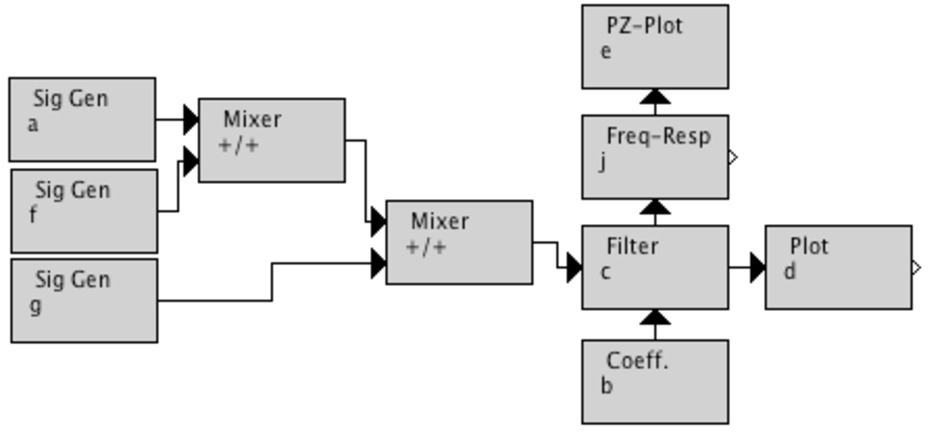
\includegraphics[width=4in]{lab6/threeinputproblem} 
   \caption{An example diagram for use in problem 2.5}
   \label{fg:threeinput}
\end{figure}
	
\paragraph{Step 2.5} Use J-DSP to determine the output of the filter \{1/3,1/3,1/3\}, $n=\{0,1,2\}$ for the
	input:
	\begin{equation}
	  x[n] = 4 + \sin[0.25\pi(n-1)] - 3 \sin[(2\pi/3)n]  
	\end{equation}
	An example diagram can be seen in Figure \ref{fg:threeinput}. Include an image 
	of the J-DSP block diagram with plots of the filter
	input and output in your report. Is the result expected? Why or why
	not?
	
	

\paragraph{Step 2.6} Create your own \block{UserDefinedFun} block to implement convolution in J-DSP. 
	To test your function, make sure it works exactly like the \block{Filter} block in J-DSP.
	Use the diagram in Figure \ref{fg:userdefined} to plot the difference between your function output and the \block{Filter} block output.
	Use the filter \{1/3,1/3,1/3\}, $n=\{0,1,2\}$ from step 2.5.
	Note: refer to section \ref{sec:example} for how to use the \block{UserDefinedFun} block in J-DSP.
	
	\begin{figure}[t]
	    \begin{center}	     
	        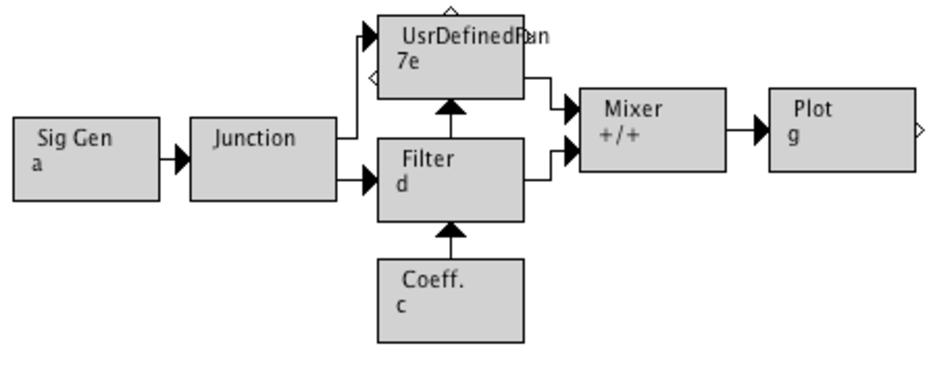
\includegraphics[width=4in]{lab6/userdefinedtest}
	        \caption{A diagram to plot the difference between \block{UserDefinedFun}
	         function output and the \block{Filter} block output for use in step 2.6.}
	         \label{fg:userdefined}
	    \end{center}
	  \end{figure}
	  
	  

\subsection{Canceling Sinusoidal Components}

Filters can be designed to cancel sinusoids.  Construct a filter in
J-DSP with the following impulse response:
\begin{equation}
h[n] = \delta[n] - 2\cos(\pi/4) \delta[n-1] + \delta[n-2]
\end{equation}

\paragraph{Step 3.1} Plot the frequency response for this filter. What
	are the zero locations?


\paragraph{Step 3.2} Use as an input to this filter the signal $x[n] =
	\sin\hat{\omega}n$, using the two frequencies $\hat{\omega} = \pi/2$
	and $\hat{\omega} = \pi/4$. Simulate the filter in J-DSP for each of
	these two inputs. Plot the filter output for each. When do we get
	cancellation?

\paragraph{Step 3.3} Can you modify the filter coefficients to cancel
	the other sinusoid? If so, show your work.


\subsection{Example User Defined J-DSP Function}\label{sec:example}
Open J-DSP and navigate to the \option{Advanced} function set. There
is one block called \block{UserDefinedFun}. Place it now and double
click to open the dialog.  You will see a dialog with example text for
a prototype java class.  In particular the class will look like:
\begin{lstlisting}
public void myCode(double[]x1,double[]x2, double[]y1, double[]y2,
		double[]b1,double[]a1, double[]b2, double[]a2, 
		double para1, double para2, double para3)
{
  //                            /\(3)
  //                --------------------           
  //           (0)<|                    |>(4)
  //               |      BLOCK         |    
  //           (1)<|                    |>(5)
  //                --------------------           
  //                            \/(2)

  // x1, x2 - input at pin 0 and pin1
  // y1, y2 - output at pin 4 and pin5
  // b1 - FIR Coefficients of the filter at input pin 2, 
  // a1 - IIR Coefficients of the filter at input pin 2
  // b2 - FIR Coefficients of the filter at output pin 3, 
  // a2 - IIR Coefficients of the filter at output pin 3

  // Para1, Para2 and Para3 are the variables that could be used 
  // in the code and can be controlled from the block Dialog.

  // Paste your code here
  // compile the file
  // upload the .class file
}
\end{lstlisting}
You can copy this code as a prototype and create your own signal
processing algorithms!  For now, you will mainly deal with the $x$ and
$y$ arrays. Each of the arrays is of length 256.  You can access this
like a any regular array in java, {\it x1.length=256}. We also have
access to four variable length arrays, {\it a1 a2 b1 b2} which contain
any filter coefficients as inputs or outputs to the function.

Lets start by creating our own .java file. Copy the example code on
the next page and save it as a .java file using your favorite java
text editor or plain text editor. The example code creates a weighted
sum of the entries in each index of {\it x1}. Namely, it goes through
each value of {\it x1} and uses the {\it b1} filter coefficients to
weight and sum the value into {\it y1}. Save the file as
``MyFunction1.java'' and then compile the file using your favorite
compiler tool for java (javac from the command line works fine for
linux and mac or The Java SE Development Kit 6 (JDK 6) can be used in
windows). This creates ``MyFunction1.class.''

After compiling, remember where you saved the ``MyFunction1.class''
compiled file. You will need to tell J-DSP where the file is
located. Go back to the J-DSP block diagram and press
\button{open}. Navigate to the ``MyFunction1.class'' compiled file and
press \option{open}. That's it! J-DSP will automatically use the
function when you attach inputs and outputs. To test the function we
just made you can connect a \block{SigGen} block to the top left pin
and a \block{Coeff} pin to the bottom as shown on page
\pageref{fg:userdefexample}. You should see a weighted sum of the
input when you plot the output. You should be able to change the
output by changing the weighting coefficients from \block{Coeff}. In
the example on page \pageref{fg:userdefexample} we are taking a
weighted sum (using the weights in {\it b1}) of each coefficient in
{\it x1} three times.  You are now ready to start developing your own
functions in J-DSP!

\begin{lstlisting} 
public class MyFunction1
{
  public void myCode(double[]x1,double[]x2, double[]y1, double[]y2,
      double[]b1,double[]a1, double[]b2, double[]a2, 
      double para1, double para2, double para3)
  {
    //                            /\(3)
    //                --------------------           
    //           (0)<|                    |>(4)
    //               |      BLOCK         |    
    //           (1)<|                    |>(5)
    //                --------------------           
    //                            \/(2)
		
    // x1, x2 - input at pin 0 and pin1
    // y1, y2 - output at pin 4 and pin5
    // b1 - FIR Coefficients of the filter at input pin 2, 
    // a1 - IIR Coefficients of the filter at input pin 2
    // b2 - FIR Coefficients of the filter at output pin 3, 
    // a2 - IIR Coefficients of the filter at output pin 3
		
    // Para1, Para2 and Para3 are the variables that could be used 
    // in the code and can be controlled from the block Dialog.
		
    for( int i = 0 ; i < 256 ; i++)
    {
      y2[i] = 0;
      for(int j=0 ; j < b1.length ; j++)
      {
        y2[i] += x1[i]*b1[j];
      }
			
    }
    // Paste your code here
    // compile the file
    // upload the .class file
  }
}
\end{lstlisting}

 \begin{figure}[h]
    \begin{center}     
        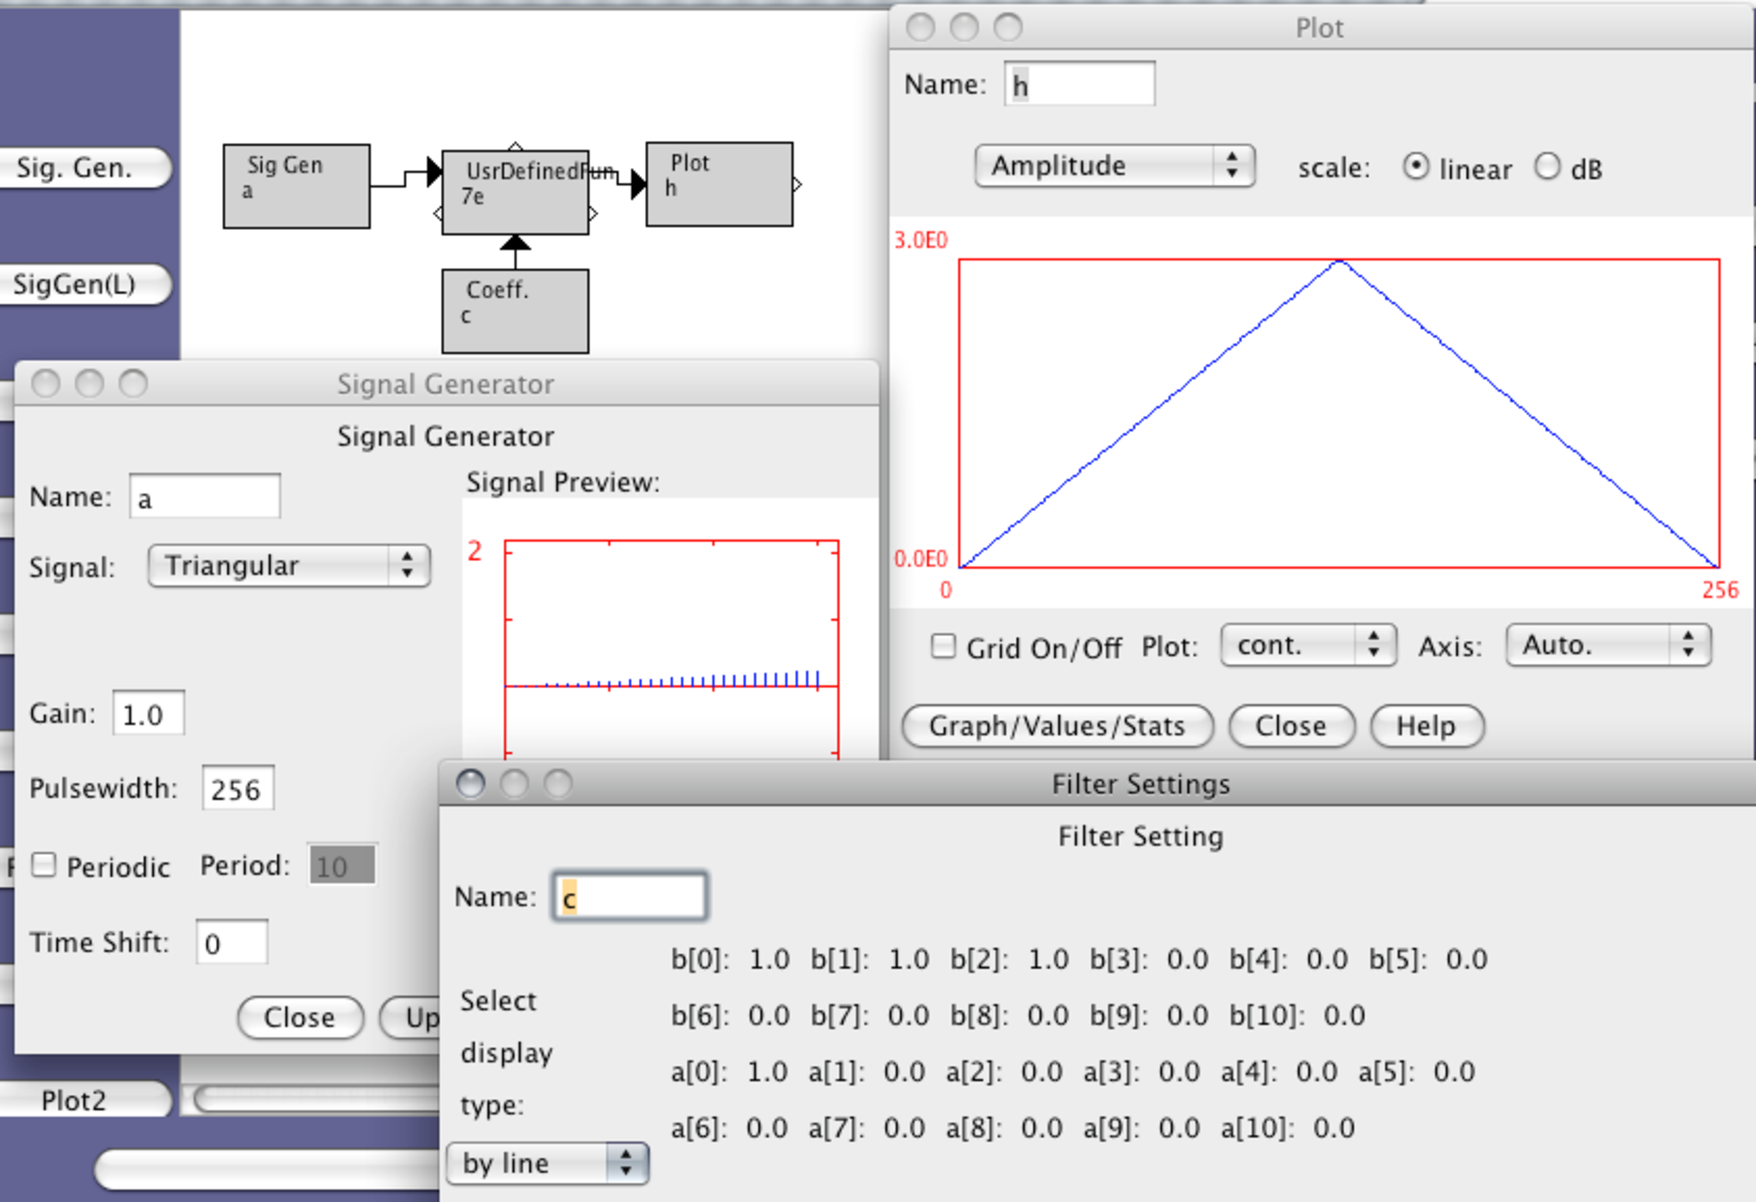
\includegraphics[width=6in]{lab6/function1examplewithplot}
        \caption{The result of using the weighted sum example code in J-DSP.}
    \end{center}
    \label{fg:userdefexample}
  \end{figure}

\subsection{Bonus: More $z$-Transforms and Convolutions}

The following properties of the $z$-transform may be useful here:

\begin{center}
\begin{tabular}{|l|c|c|} \hline
Property      & Time Domain, $Z^{-1}\{\cdot\}$ & z-Domain, $Z\{\cdot\}$ \\ \hline\hline
Linearity     & $a_1x[n]+a_2y[n]$ & $a_1X(z)+a_2Y(z)$\\ 
Time shift    & $x[n-k]$       & $z^{-k}X(z)$\\ 
Scaling in the z-domain 
              & $a^nx[n]$        & $X(a^{-1}z)$ \\ 
Time reversal & $x[-n]$        & $X(z^{-1})$\\ 
Differentiation in the z-domain 
              & $nx[n]$          & $-z \deriv{X(z)}{z}$ \\ 
Convolution   & $x[n] \ast y[n]$       & $X(z)Y(z)$ \\ \hline
\end{tabular}
\end{center}



\paragraph{$z$-Transform of arbitrary sequences}
Give the $z$-transform of the following sequences, $x[n]$ (assume
$x[n]=0$ for all $n$ not stated):
\begin{enumerate}
\item $x[n]=\{2, 4, 6, 4, 2\}$, $n = \{0, 1, 2, 3, 4\}$

\item $x[n] = \delta[n]$

\item $x[n] = \delta[n-1]$

\item $x[n] = 2\delta[n] - 3\delta[n-1] +4\delta[n-3]$

\item $x[n] = 2\delta[n] + 4\delta[n-1] + 6\delta[n-2] + 4\delta[n-3] + 2\delta[n-4]$
\end{enumerate}


\paragraph{Inverse $z$-transforms}
Give the inverse $z$-transform of $H(z) = 1 + 5z^{-1} - 3z^{-2} +
2.5z^{-3} +4z^{-8}$.

\paragraph{Transfer function \& impulse response}
Give the transfer function and impulse response for a filter with
zeros at $(r, \hat{\omega}) = \{(1, 0), (1, \pm \pi/2), (0.9, \pm
\pi/3)\}$.

% LocalWords:  WebQ MATLAB DSP

%&LaTeX

\section{Joe Fourier Was Not a Discrete Fellow}

\subsection{Lab Background}
By the end of this lab you should have a firm understanding of how the
Discrete Fourier Transform (DFT) can be implemented exactly using the
Fast Fourier Transform (FFT). In addition you should be able to
identify common problems using the DFT to analyze signals. You will
also be familiar with a new tool, the spectrogram, that uses the DFT
as a function of time.

\subsection{Implementing the DFT}

Recall that the DFT can be implemented directly from the analysis
equation. For a length $N$ signal $x[n]$,
\begin{align}
X[k]=\sum_{n=0}^{N-1}x[n]e^{-j \frac{2\pi}{N} nk} && \text{for $k = 0, 1, 2, \cdots N-1$}
\label{eq:dft}
\end{align}
The order of the implementation is $O(N)=N^2$. The following Java code
outlines implementation of a 256-point DFT. It is written without any
algorithmic speedup (i.e., it exactly mirrors equation \ref{eq:dft}).
\begin{lstlisting}[language=Java,basicstyle=\mlttfamily\small]
public class MyDFT
{
  // x is the input and y is the magnitude of the complex DFT
 public void computeDFT(double[] x, double[] y)
  {
  double[] yImag = new double[256];
  double[] yReal = new double[256];

  double twoPiOverN = 2*Math.PI/256;

  for (int k = 0 ; k < 256 ; k++)
  {
    yReal[k] = 0;
    yImag[k] = 0;
    for (int n = 0 ; n < 256 ; n++)
    {
      yReal[k] += x[n]*Math.cos(n*k*twoPiOverN);
      yImag[k] += -x[n]*Math.sin(n*k*twoPiOverN);
    }
    y[k] = Math.sqrt(yReal[k]*yReal[k] + yImag[k]*yImag[k]);
  }
 }
}
\end{lstlisting}

Note that, unlike in Matlab, there is no native support in Java for
complex numbers so this arithmetic is written out explicitly in the
code above. For example, the equation $y=x\times e^{a}$ (where x is a
real number) must be explicitly written out using Euler's formula, and
the real and imaginary portions saved in separate variables,
$y_{real}=x\times \cos(a)$ and $y_{imag}=x\times \sin(a)$.

The FFT algorithm can be used to reduce the computation time of the
DFT to $O(N)=N\log_2 N$ --- a significant speedup for even modest
length signals.

\subsection{The FFT in Matlab}

Matlab includes a \verb|fft| function (there are many more related
operations in the Signal Processing Toolbox, but we are sticking to
``vanilla'' Matlab here). You can look at the documentation for this
function; pay especial attention to the frequency values that
correspond to each element of the vector that this function returns,
and to how to specify the number of points in the FFT it computes.

\paragraph{Step 1.1} Implement your own \verb|myFFT| function in
Matlab that takes a real-valued vector as input, computes a 256-point
FFT, and returns a real-valued vector that is the magnitude of the
(single-sided, i.e., only positive frequencies) FFT. Implement this
function using loops (i.e., do not use recursion). The first part of
this code performs a bit reversal on the input array. You can use the
following code to perform the bit reversal efficiently (efficient bit
reversal algorithms in other languages are typically more complex):
\begin{lstlisting}[style=Matlab-editor,basicstyle=\mlttfamily\small]
% Assume that you want to do a bit reversal of the contents of the vector x
indices = [0 : length(x)-1];                 % binary indices need to start at zero
revIndices = bin2dec(fliplr(dec2bin(indices, 8))); % bit reversed indices
revX = x(revIndices+1);                      % Add 1 to get Matlab indices
\end{lstlisting}
This code converts the vector of in-order indices to an array of
8-character strings (representing those indices as binary 8-bit
numbers). Each string is then reversed, and converted back to
numbers. The resultant vector of indices (which is what they are after
we add one to each) is applied to the signal to pull its entries out
into a new vector, with the order of the entries in bit-reversed
order.

Once you've done this, all you need to do is iterate over the array
$\log_2 N$ times! Remember that you're performing complex arithmetic
and to compute the magnitude of the output array once the FFT is
computed. Include a copy of your Matlab code in your report.

\paragraph{Step 1.2} 
Check your results using the Matlab \verb|fft| function. Your results
should be quite similar, if not identical; this should be apparent by
comparing graphs of the outputs. Take the FFT of a sinusoid with a
frequency of $\pi/4$ radians per second using your FFT implementation
and the \verb|fft| function.

\paragraph{Step 1.3}
Prove that the number of complex multiplies performed by your code is
$O(N \log N)$.

\subsection{Using the DFT}

\paragraph{Step 2.1} 
Create a sum of two sinusoids. Use the built-in Matlab \verb|fft|
function (it will allow you, among other things, to apply an $n$-point
FFT to a signal with more than $n$ samples) to compute the FFT of the
sum and then plot the FFT magnitude. Use frequencies of $0.13\pi$ and
$0.19\pi$ for the two sinusoids. Make sure that there are at least 256
samples in each waveform, as you'll want to use a 256-point FFT! Also,
make sure you correctly compute the corresponding frequency values
(either from 0 to $\pi$ or $-\pi$ to $\pi$, depending on whether you
prefer plotting the single-sided magnitudes or not) for the FFT
X-axis, and label it appropriate in your graph. What does the result
look like? Does this make sense?


\paragraph{Step 2.2} At what index (or indices) does the FFT magnitude
reach its peak value(s)? What frequency (or frequencies) does this
correspond to?


\paragraph{Step 2.3} Change the frequencies of the sinusoids to
$0.13\pi$ and $0.14\pi$. Repeat steps 2.1 and 2.2. Do the results
still make sense?


\paragraph{Step 2.4} Replace the sum of two sinusoids with your
\verb|DTMFCoder| function from lab 6. Input a selection of button
values. Do the FFT function and plot show the separate frequencies for each
button?



\subsection{Spectrograms}

Comparing FFT graphs (as in the step 2.4 above) can be difficult to
do. But what if we could analyze the frequency content of a signal as
a function of time? That would make it easier to see differences in
frequency if a signal started changing (like a string of DTMF keys
pressed in turn). To do this we will need a new tool called the
\emph{Spectrogram}. The spectrogram is simply an algorithm for
computing the FFT of a signal at different times and plotting them as
a function of time. The spectrogram is computed in the following way:

\begin{enumerate}
\item A given signal is ``windowed.'' This means that we only take a
  certain number of points from the signal (for this example assume we
  are using a window of length 128 points). To start out, we take the
  first 128 points of the signal (points 1 through 128 of the input
  vector).
\item Take the FFT of the window and save the it in a separate array.
\item Advance the window in time by a certain number of points. For
  instance we can advance the window by 64 points so that we now have
  a window of indices 65 through 192 from the input signal array.
\item Repeat steps 1--3, saving the FFT of each window, until there
  are no longer any points in the input array.
\item Form a 2-D matrix whose columns are the FFT magnitudes of each
  window (placed in chronological order). In this way, each row
  represents a certain frequency, each column represents a given
  instant in time, and the value of the matrix represents the
  magnitude of the FFT.
\end{enumerate}

The result is called a \emph{spectrogram} and is usually displayed as
an RGB image where blue represents small FFT magnitudes and red
represents larger FFT magnitudes (the \emph{Jet} colormap if you are
familiar with color visualizations). There is an art to choosing the
correct parameters of the spectrogram (i.e., window size, FFT size,
how many points to advance the FFT, etc.). Each parameter has
tradeoffs for the time and frequency resolution of the resulting
spectrogram. For our purposes here, we will not be concerned with
these tradeoffs. Instead we will be more interested in getting
familiar with analysis using spectrograms.

The Matlab Signal Processing Toolbox has a \verb|spectrogram|
function, but you can retrieve a drop-in replacement for it from
\url{http://www.ee.columbia.edu/ln/rosa/matlab/sgram/} that will work
without that toolbox. See the online Matlab documentation for the
\verb|spectrogram| function to understand what the parameters to that
function are (though, for our purposes, you should just be able to use
the call \verb|y = myspecgram(x)|.

\paragraph{Step 3.1} Use your \verb|DTMFCoder| function again. Instead
of computing its FFT, compute its spectrogram instead. What does the
spectrogram look like for button 1? Are both frequencies present?


\paragraph{Step 3.2} For this step, use \verb|DTMFCoder| to generate
the codes for multiple buttons --- at least three --- and concatenate
them together to form a single vector. Does the spectrogram make it
easier to judge the frequency content of the keys? Can you clearly see
when the signal changes from one key to another?

% LocalWords:  WebQ MATLAB DSP

%&LaTeX

\section{Discrete Fourier Transform}

\subsection{Lab Background}
By the end of this lab you should have a firm understanding of how the
Discrete Fourier Transform (DFT) can be implemented exactly using the
Fast Fourier Transform (FFT). In addition you should be able to
identify common problems using the DFT to analyze signals. You will
also be familiar with a new tool, the spectrogram, that uses the DFT
as a function of time.

\subsection{Implementing the DFT}

% TODO: have them work with this block for a good implementation of the J-DSP
Recall that the DFT can be implemented directly from the analysis
equation. For a length $N$ signal $x[n]$,
\begin{align}
X[k]=\sum_{n=0}^{N-1}x[n]e^{-j \frac{2\pi}{N} nk} && \text{for $k = 0, 1, 2, \cdots N-1$}
\label{eq:dft}
\end{align}
The order of the implementation is $O(N)=N^2$. The following java code
can be used to implement the DFT in J-DSP. It is implemented without
any algorithmic speedup (i.e., it exactly mirrors equation
\ref{eq:dft}).  Example of raw DFT implementation:
	\begin{lstlisting}
public class MyFunction1
{
 public void myCode(double[]x1,double[]x2,double[]y1,double[]y2,
 	double[]b1,double[]a1,double[]b2,double[]a2,
 	double para1, double para2, double para3)
  {
  // x1, x2 - input at pin 0 and pin1
  // y1, y2 - output at pin 4 and pin5
  // raw DFT implementation
  double[] yImag;
  double[] yReal;
  yImag = new double[256];
  yReal = new double[256];
  double twoPiOverN = 2*Math.PI/256;
  for( int k = 0 ; k < 256 ; k++)
  {
    yReal[k] = 0;
    yImag[k] = 0;
    for( int n = 0 ; n < 256 ; n++)
    {
      yReal[k] += x1[n]*Math.cos(n*k*twoPiOverN);
      yImag[k] += -x1[n]*Math.sin(n*k*twoPiOverN);
    }
    y1[k] = Math.sqrt(yReal[k]*yReal[k]+yImag[k]*yImag[k]);
  }
 }
}
	\end{lstlisting}
Note that there is not a native support in java for complex numbers so
this arithmetic is written out explicitly in the code above. For
example, the equation $y=x\times e^{a}$ (where x is a real number)
must be explicitly written out using Euler's formula, and the real and
imaginary portions saved in separate variables, $y_{real}=x\times
\cos(a)$ and $y_{imag}=x\times \sin(a)$.

The FFT algorithm, on the other hand, can be used to reduce the
computation time of the DFT to $O(N)=N\log_2 N$ - a significant
speedup for even modest length signals.

\paragraph{Step 1.1}
Write some example code to multiply \emph{two} complex numbers,
$c=a\times b$. Remember to represent the variables by their real and
imaginary parts and save the real and imaginary parts in separate
variables.


\paragraph{Step 1.2} 
Use the \block{UserDefinedFun} block to implement the FFT using loops
(i.e., do not use recursion). The first part of this code performs a
bit reversal on the input array. Use the following code to perform the
bit reversal:
% make more explict, bit rev vrbl
\begin{lstlisting}
// bit reversal
int  index;
int  N = 256;
double[] reversedX1 = new double[256];
// need to shift 32 bit integer to make it an 8 bit reversal
int shift = (32-(int)Math.round(Math.log(N)/Math.log(2))); 
for( int n = 0 ; n < N ; n++){
  index = (Integer.reverse(n))>>>shift; //reverse and then shift down to 8 bit
  reversedX1[n] = x1[index]; 
}
\end{lstlisting}
Then iterate over the array $\log_2 N$ times! Remember to explicitly
carry out any complex arithmetic and take the magnitude of the output
array once the FFT is computed. Include a copy of the java code in
your report.

\paragraph{Step 1.3} 
Check your results in J-DSP using the \block{FFT} block. Your results
should be identical. Take the FFT of a sinusoid with a frequency of
$\pi/4$ radians per second using your FFT implementation and the
\block{FFT} block provided in J-DSP. Include a screenshot of the
output plots.



\subsection{Using the DFT}
% switch over to spectrogram example with DTMF - organize introduction
% for ease of use over multiple steps
\paragraph{Step 2.1} 
Create a sum of two sinusoids in J-DSP. Use the \block{FFT} block to
compute the FFT of the sum and then plot the FFT magnitude. Use a
frequency of $0.13\pi$ and $0.19\pi$ for the two sinusoids. Make sure
that the \option{pulsewidth} for each is set to 256. What does the
result look like? Does this make sense?


\paragraph{Step 2.2} At what index (or indices) does the FFT magnitude
reach its peak value(s)? What frequency (or frequencies) does this
correspond to?


\paragraph{Step 2.3} Change the frequencies of the sinusoids to
$0.13\pi$ and $0.14\pi$. Repeat steps 2.1 and 2.2. Do the results
still make sense?


\paragraph{Step 2.4} Replace the sum of two sinusoids in J-DSP with
the \block{DTMF} block under the \menu{Audio Effects} function
list. Press some of the keys in the \block{DTMF} block. Does the FFT
block show separate frequencies for each button?



\subsection{Spectrograms}
Comparing FFT graphs (as in the step 2.4) can be difficult to do. But
what if we could analyze the frequency content of a signal as a
function of time? That would make it easier to see differences in
frequency if a signal started changing (like a string of DTMF keys
pressed in turn). To do this we will need a new tool called the
\emph{Spectrogram}. The spectrogram is simply an algorithm for
computing the FFT of a signal at different times and plotting them as
a function of time. The spectrogram is computed in the following way:

\begin{enumerate}
\item A given signal is ``windowed.'' This means that we only take a
  certain number of points from the signal (for this example assume we
  are using a window of length 128 points). To start out, we take the
  first 128 points of the signal (points 0 through 127 of the input
  array).
\item Take the FFT of the window and save the it in a separate array.
\item Advance the window in time by a certain number of points. For
  instance we can advance the window by 64 points so that we now have
  a window of indices 64 through 191 from the input signal array.
\item Repeat steps 1-3, saving the FFT of each window, until there are
  no longer any points in the input array.
\item Form a 2-D matrix whose columns are the FFT magnitudes of each
  window (placed in chronological order). In this way, each row
  represents a certain frequency, each column represents a given
  instant in time, and the value of the matrix represents the
  magnitude of the FFT.
\end{enumerate}

The result is called a Spectrogram and is usually displayed as an RGB
image where blue represents small FFT magnitudes and red represents
larger FFT magnitudes (the \emph{Jet} colormap if you are familiar
with color visualizations). There is an art to choosing the correct
parameters of the spectrogram (i.e., window size, FFT size, how many
points to advance the FFT, etc.). Each parameter has tradeoffs for the
time and frequency resolution of the resulting spectrogram. For our
purposes here, we will not be concerned with these tradeoffs. Instead
we will be more interested in getting familiar with analysis using
spectrograms.

\paragraph{Step 3.1} Use the DTMF setup from step 2.4. Instead of
using the \block{FFT} block, use the \block{Spectrogram} block under
the \menu{Statistical DSP} function stack. Keep all parameters in the
\block{Spectrogram} set to the default. Set the \block{DTMF} block to
play five frames per key press. Press the number ``1.'' What does the
spectrogram look like? Are both frequencies present?


\paragraph{Step 3.2} Now set the \block{DTMF} block to
\option{Record}. Also set the \option{Resolution} parameter inside the
\block{Spectrogram} block to 4 or 8 (otherwise you may notice a lag
for updating the spectrogram - it can be considerably CPU intensive
for large input signals). The \option{Resolution} parameter controls
how many points the sliding window advances at each time step (larger
steps mean we take fewer FFTs). Press each key in the \block{DTMF}
block in turn. Does the spectrogram make it easier to judge the
frequency content of the keys? Include a screenshot for your report.

% LocalWords:  WebQ MATLAB DSP



\end{document}
% LocalWords:  MATLAB
